\documentclass[12pt,a4paper]{report}
\usepackage[utf8]{inputenc}
\usepackage{geometry}
\usepackage{mathptmx} % Times New Roman font to match the template
\usepackage{tabularx}
\usepackage{graphicx}
\usepackage{array}
\usepackage{tocloft}
\usepackage{titlesec}
\usepackage{hyperref}
\usepackage{enumitem}
\usepackage{float}
\usepackage[skip=6pt plus 1pt minus 1pt]{parskip}

% Balanced 1-inch margins all around; zero paragraph indentation
\geometry{
    top=1in,
    bottom=1in,
    left=1in,
    right=1in
}
\setlength{\parindent}{0pt}

% Stop LaTeX from stretching vertical whitespace between paragraphs
\raggedbottom

% Uniform tight list spacing
\setlist{topsep=3pt, itemsep=2pt, partopsep=0pt, parsep=0pt}

% Uniform float spacing around figures
\setlength{\floatsep}{8pt plus 2pt minus 2pt}
\setlength{\textfloatsep}{10pt plus 2pt minus 2pt}
\setlength{\intextsep}{8pt plus 2pt minus 2pt}

% Dotted lines in TOC for all section levels
\renewcommand{\cftsecleader}{\cftdotfill{\cftdotsep}}
\renewcommand{\cftsubsecleader}{\cftdotfill{\cftdotsep}}
\renewcommand{\cftsubsubsecleader}{\cftdotfill{\cftdotsep}}

% Numbering and TOC depth down to subsubsection (4.1.1)
\setcounter{secnumdepth}{3}
\setcounter{tocdepth}{3}

% Strictly map sections to 1, 1.1, 1.1.1 (removes chapter 0 prefix from report class)
\renewcommand{\thesection}{\arabic{section}}
\renewcommand{\thesubsection}{\thesection.\arabic{subsection}}
\renewcommand{\thesubsubsection}{\thesubsection.\arabic{subsubsection}}

% Format chapter/section headers to clean numbered titles
\titleformat{\section}{\fontsize{14pt}{18pt}\bfseries}{\thesection}{1em}{}
\titleformat{\subsection}{\fontsize{12pt}{15pt}\bfseries}{\thesubsection}{1em}{}
\titleformat{\subsubsection}{\fontsize{11pt}{14pt}\bfseries}{\thesubsubsection}{1em}{}

\hypersetup{
    colorlinks=true,
    linkcolor=black,
    urlcolor=blue,
    citecolor=black
}

\begin{document}

% ----------------------------------------------------------------------
% TITLE PAGE
% ----------------------------------------------------------------------
\begin{titlepage}
    \centering

    % 1. Full Project Title
    \vspace*{0.3cm}
    {\fontsize{18pt}{22pt}\selectfont \textbf{Multi-Organ Disease Classification and Segmentation with Clinical Decision Support, Report Generation and 3D Visualization as Assistive Modules}}\\[1.2cm]

    % 2. Document Identifier
    {\fontsize{16pt}{20pt}\selectfont Software Requirement Specifications}\\[0.8cm]

    % 3. Degree Program
    {\fontsize{14pt}{18pt}\selectfont Bachelor of Science in Computer Science}\\[0.8cm]

    % 4. By Section
    {\fontsize{13pt}{16pt}\selectfont By}\\[0.6cm]

    % 5. Students Table (Solo)
    \renewcommand{\arraystretch}{1.5}
    \begin{tabularx}{\textwidth}{|c|>{\centering\arraybackslash}p{3.5cm}|>{\centering\arraybackslash}p{3.2cm}|>{\centering\arraybackslash}p{2.8cm}|>{\centering\arraybackslash}X|}
        \hline
        \textbf{\#} & \textbf{Name} & \textbf{Registration \#} & \textbf{Mobile \#} & \textbf{E-Mail} \\
        \hline
        1 & Muhammad Fezan & Fall-23-BSCS-466 & 03097413565 & fa-23-bscs-466@lgu.edu.pk \\
        \hline
    \end{tabularx}

    \vspace{2.2cm}

    % 6. Supervised by & Co-Supervised by
    \noindent
    \begin{minipage}{0.48\textwidth}
        \centering
        \textbf{Supervised by}\\[1.5cm]
        \underline{\hspace{5cm}}\\[0.2cm]
        Miss Naila Noreen
    \end{minipage}
    \hfill
    \begin{minipage}{0.48\textwidth}
        \centering
        \textbf{Co-Supervised by}\\[1.5cm]
        \underline{\hspace{5cm}}\\[0.2cm]
        Abdul Qayyum
    \end{minipage}

    \vfill

    % 7. Centered University Logo at Bottom
    \includegraphics[width=2.8cm]{lgu_logo.jpg}\\[0.6cm]

    % 8. Department, University, Location
    {\fontsize{14pt}{18pt}\selectfont Department of Computer Science}\\[0.2cm]
    {\fontsize{14pt}{18pt}\selectfont Lahore Garrison University}\\[0.2cm]
    {\fontsize{14pt}{18pt}\selectfont Lahore}

\end{titlepage}

% ----------------------------------------------------------------------
% TABLE OF CONTENTS
% ----------------------------------------------------------------------
\newpage
\pagenumbering{roman}
\tableofcontents
\newpage
\pagenumbering{arabic}
\setcounter{page}{4} % Matches starting page from template

% ----------------------------------------------------------------------
% 1. INTRODUCTION
% ----------------------------------------------------------------------
\section{Introduction}

\subsection{Purpose}
This document specifies software requirements specifications for OpenMed, a multi-organ disease classification and segmentation platform with Clinical Decision Support, Report Generation and 3D Visualization as Assistive Modules. It covers release 1.0 in full. That includes how the image passes through different stages, the classification models that predict the disease with confidence scores and Grad-CAM explanations, the segmentation models that pinpoint the exact location of the region of interest, the assistive prompting tools, the report generation, the decision support assistant and the 3D anatomy of the organs covered.

Developers, project evaluators and supervisors use this document as the baseline to verify the system design and the performance benchmarks before deployment.

\subsection{Document Conventions}
The document follows the departmental SRS template which itself is an adaptation of the IEEE 830 recommended practice for software requirements specifications as popularized by Wiegers. Sections 1 to 3 describe the product from the outside, Section 4 provides the functional requirements feature by feature, and Section 5 states the non-functional requirements and the detailed subsystem design. Figures are numbered sequentially and all carry descriptive captions.

\subsection{Intended Audience and Reading Suggestions}
The document has six audiences with different needs. The table below states what each should read first; a reader who has time for only one section should read Section 1.4 first, since it states what the product is and what it does not cover.

\vspace{0.2cm}
\noindent
\renewcommand{\arraystretch}{1.3}
\begin{tabularx}{\textwidth}{|>{\raggedright\arraybackslash\bfseries}p{3.2cm}|>{\raggedright\arraybackslash}X|>{\raggedright\arraybackslash}p{3.8cm}|}
\hline
\textbf{Reader} & \textbf{Why they are reading} & \textbf{Suggested sequence} \\
\hline
Supervisor and evaluation committee & Judge whether the scope is coherent, achievable and correctly bounded. & 1.1 $\rightarrow$ 1.4 $\rightarrow$ 2.2 $\rightarrow$ 4 (headings) $\rightarrow$ 5.1 $\rightarrow$ 5.2 \\
\hline
Backend developer & Implement or extend the service without breaking the model contracts. & 2.4 $\rightarrow$ 2.5 $\rightarrow$ 3.3 $\rightarrow$ 4 $\rightarrow$ 5.1 $\rightarrow$ 5.6 \\
\hline
Frontend developer & Build screens against a stable response shape and a defined error model. & 3.1 $\rightarrow$ 3.3 $\rightarrow$ 3.4 $\rightarrow$ 4.1 $\rightarrow$ 4.7 \\
\hline
Test engineer & Derive acceptance tests from stated requirements rather than from the code. & 4 (all) $\rightarrow$ 5.1 $\rightarrow$ 5.3 $\rightarrow$ 5.4 \\
\hline
Radiologist or clinical reviewer & Understand what the system claims, what it refuses to claim, and where the human stays in control. & 1.4 $\rightarrow$ 2.2 $\rightarrow$ 3.1 $\rightarrow$ 5.2 $\rightarrow$ 5.5 \\
\hline
ML engineer & Publish a checkpoint that the service will accept on first load. & 2.5 $\rightarrow$ 3.3.2 $\rightarrow$ 5.1 $\rightarrow$ 5.6.2 \\
\hline
\end{tabularx}
\vspace{0.2cm}

\subsection{Product Scope}
OpenMed builds a medical diagnostic system that combines disease detection, tumor tracing, and clinical reports into one simple platform. The project scope targets a minimum of ten distinct organ systems including Heart, Brain, Kidney, Blood, Bones, Eyes, Lungs, Liver, Skin, and Pancreas as the committed core, with the system designed in such a way that it can add further organs beyond this set. For each organ, the core models name the illness and trace the exact shape of the damaged area on the scan.

To handle complex diagnoses accurately, the system uses a mixture of experts approach where two models check disease findings and general abnormalities side by side. For boundary tracing, automated models outline the detected problem, but because automated tools can sometimes miss subtle edges or secondary abnormalities, OpenMed integrates MedSAM-2 as a generic assistive module. This runs across any organ. The doctor can click a point or draw a box around an abnormal region on the scan to trigger immediate prompt-based re-segmentation.

A clean dashboard turns all model outputs into structured patient reports and 3D views of the organs. The built-in clinical assistant lets doctors ask questions directly about the case, with answers tied strictly to the scan results. The whole system runs as a web app, letting doctors inspect patient scans in a normal web browser on standard computer hardware, without needing expensive server racks.

% ----------------------------------------------------------------------
% 2. OVERALL DESCRIPTION
% ----------------------------------------------------------------------
\section{Overall Description}

\subsection{Product Perspective}
OpenMed is a new, self-contained web platform designed to replace the fragmented software tools currently used in hospital diagnostic workflows. In standard clinical setups, doctors have to juggle multiple disconnected applications: a viewer for scan slices, single-organ research tools that do not talk to each other, separate software for 3D views, plus manual templates for reports. OpenMed brings all of these steps into one system.

The product targets the practical bottlenecks in medical imaging, particularly in resource-limited regions like Pakistan where a shortage of radiologists causes long patient delays. Most existing medical AI solutions fail to get used in real clinics because they focus on only one body part, output a single disease name without showing where the damaged area is, and dump an answer without helping with the rest of the workflow. Doctors still end up checking every slice by hand and drafting reports from scratch.

OpenMed operates as a complete assistive workstation inside a standard web browser. The system connects the frontend diagnostic workspace to a modular backend where each organ has its own dedicated data handling and inference pipeline. New organ modules can then be added on the same stack without tangling the platform. Once a scan is analyzed, the classification findings, automated segmentation masks, and interactive MedSAM-2 prompt corrections flow directly into the structured report generator, the 3D organ viewer, and the clinical Q\&A assistant. The platform runs inference on standard computer hardware with consumer CPUs, so it does not depend on expensive hospital GPU servers.

\subsection{Product Functions}
OpenMed provides a unified set of diagnostic functions across the clinical workflow. The major functions include:

\begin{itemize}[leftmargin=1.2em]
    \item \textbf{Medical Scan Ingestion and Preprocessing:}
    \begin{itemize}[leftmargin=1.2em]
        \item Allows clinicians to upload standard medical scans (such as MRI, CT, and X-ray images) through a simple browser interface.
        \item Validates scan dimensions, normalizes pixel intensities, and confirms scan orientation before running any model.
    \end{itemize}
    \item \textbf{Disease Classification via Mixture of Experts:}
    \begin{itemize}[leftmargin=1.2em]
        \item Identifies specific illnesses and abnormalities across multiple supported organ systems.
        \item Combines two complementary models where needed to cross-check specific disease conditions alongside general radiological findings.
        \item Generates calibrated confidence scores so doctors can see how certain the system is about each finding.
    \end{itemize}
    \item \textbf{Automated and Assistive Segmentation:}
    \begin{itemize}[leftmargin=1.2em]
        \item Automatically outlines the exact boundaries of damaged tissue or tumors on the scan slices.
        \item Provides interactive prompt-based re-segmentation using MedSAM-2 across any supported organ, letting the doctor click a point or draw a box to fix missed borders or secondary lesions.
        \item Calculates quantitative measurements including affected area and volume from the resulting masks.
    \end{itemize}
    \item \textbf{Interactive 3D Anatomy Visualization:}
    \begin{itemize}[leftmargin=1.2em]
        \item Renders interactive 3D organ models inside the web browser using WebGL.
        \item Overlays the segmented damaged areas directly onto the 3D organ model so clinicians can inspect depth, size, and spatial orientation.
        \item Provides full camera controls including rotation, zoom, pan, and layer opacity adjustment.
    \end{itemize}
    \item \textbf{Structured Clinical Report Generation:}
    \begin{itemize}[leftmargin=1.2em]
        \item Converts classification results, segmented region measurements, and scan metadata into a structured clinical report template.
        \item Allows doctors to review, edit, or override any automated finding before signing off.
        \item Exports finalized diagnostic reports directly to PDF.
    \end{itemize}
    \item \textbf{Clinical Decision Support Assistant:}
    \begin{itemize}[leftmargin=1.2em]
        \item Provides an integrated chat assistant where doctors can ask questions about the current case findings.
        \item Keeps answers grounded strictly in the generated scan results and clinical metrics rather than pulling random answers from external sources.
    \end{itemize}
    \item \textbf{Case Management and Audit Trail:}
    \begin{itemize}[leftmargin=1.2em]
        \item Stores patient scan sessions, segmentation masks, and generated reports for future review.
        \item Keeps track of both the initial automated outputs and the doctor's manual adjustments to maintain clear clinical accountability.
    \end{itemize}
\end{itemize}

\subsection{User Classes and Characteristics}
OpenMed defines four user classes based on clinical responsibility and system access:

\begin{itemize}[leftmargin=1.2em]
    \item \textbf{1. Radiologists and Medical Specialists (Primary User Class):} 
    Licensed specialists with high medical expertise who use the system daily during hospital reading shifts. They have full clinical authority across the workspace. They upload scans, review classification scores, inspect scan slices, place MedSAM-2 prompt points and bounding boxes to fix lesion borders, examine 3D models, and approve or modify final diagnostic reports.

    \item \textbf{2. General Physicians and Referring Doctors (Secondary User Class):}
    Medical doctors who review patient cases several times a week to plan treatments or surgical work. They do not perform scan contouring. They have read-only access to finalized reports, classification results, and 3D organ models, with permission to add clinical consultation notes and query the assistant for quick case summaries.

    \item \textbf{3. Radiology Residents and Medical Students (Tertiary User Class):}
    Trainees who use the software regularly during academic rotations to learn radiological interpretation. They operate in training mode. They can upload practice scans, test their manual observations against model outputs, explore 3D anatomy, and practice boundary selection using MedSAM-2, but cannot create or approve official patient records.

    \item \textbf{4. System and Hospital Administrators (Operational User Class):}
    IT personnel with technical systems expertise and no medical background. They access the platform occasionally for setup and maintenance. They manage user accounts, set up local storage paths, monitor CPU memory usage, and check audit logs, with no access to clinical medical judgments.
\end{itemize}


\subsection{Operating Environment}
OpenMed operates as a client-server web application with minimal hardware overhead:

\begin{itemize}[leftmargin=1.2em]
    \item \textbf{Client Environment:} Runs inside any modern web browser supporting WebGL 2.0 and WebSockets (Google Chrome 110+, Mozilla Firefox 115+, Microsoft Edge 110+, Safari 16+).
    \item \textbf{Server Environment:} The system works fine on a CPU-only machine with a 4-core processor and 8 GB of RAM; adding a dedicated GPU is an optional plus.
\end{itemize}

\subsection{Design and Implementation Constraints}
OpenMed adheres to four core constraints:

\begin{itemize}[leftmargin=1.2em]
    \item \textbf{1. Hardware Boundaries and Lazy Loading:} The system executes inference on consumer computers (4-core CPU, 8 GB RAM) without requiring a GPU. Zero model weights load on boot; only the active organ loads into memory, and switching organs unloads previous weights to keep RAM within 8 GB.
    \item \textbf{2. Assistive Workflow and Clinical Safety:} The software functions strictly as an assistive aid. All predictions and segmentation masks remain editable by the physician and require digital sign-off before official clinical use.
    \item \textbf{3. Local Execution and Data Sovereignty:} All scan processing, model inference, and report building execute locally on the host machine. Patient imaging never leaves the clinic network.
    \item \textbf{4. Modular Pipeline Isolation:} Each organ pipeline maintains independent data loaders and inference logic so nothing gets tangled. Dual-model pipelines keep preprocessing paths separate to prevent input contamination.
\end{itemize}

\subsection{User Documentation}
OpenMed provides user and technical documentation across two primary channels:

\subsubsection{Built-in Web Documentation Portal}
The running web application includes a built-in documentation portal accessible directly from the global navigation menu. This portal gives clinicians and researchers interactive reference guides for every organ module without leaving the application. It explains the underlying classification models, how the dual-model mixture of experts works for chest imaging, and how to operate interactive tools like MedSAM-2 for point and box re-segmentation. It also documents 3D WebGL viewer navigation, calibration reliability protocols, and in-app tooltips that assist doctors during active scan interpretation.

\subsubsection{GitHub Repository and Organ-Level Documentation}
Complete technical documentation and deployment guides are maintained in the official GitHub repository at \url{https://github.com/H0NEYP0T-466/OpenMed}. The root repository documents system installation, CPU runtime configuration, and test suite execution. Each organ module (such as Brain and Lungs) contains its own dedicated directory-level README detailing preprocessing rules, input tensor dimensions, and inference pipelines. These organ folders also include verifiable training logs (\texttt{train.log}), evaluation metrics (\texttt{metrics.json}, \texttt{history.csv}), ROC curves, confusion matrices, and dataset hygiene audit reports showing duplicate removal via SHA-256 and pHash alongside train/validation split manifests.

\subsection{Assumptions and Dependencies}
OpenMed operates under the following technical assumptions and system dependencies:

\begin{itemize}[leftmargin=1.2em]
    \item \textbf{1. Assumptions:}
    \begin{itemize}[leftmargin=1.2em]
        \item \textit{Scan Quality:} Uploaded medical images are assumed to be diagnostic-grade scans (frontal chest X-rays and brain MRI series) with readable contrast. Corrupted or unreadable files require re-acquisition by hospital staff.
        \item \textit{Clinician Oversight:} The software assumes operation by a trained medical professional who understands radiological terminology, reviews confidence scores critically, and verifies segmentation boundaries before signing reports.
        \item \textit{Hardware and Browser Readiness:} The backend host is assumed to meet baseline specs (quad-core CPU, 8 GB RAM), and client workstations run modern browsers with WebGL 2.0 enabled.
        \item \textit{Sequential Workflow:} The lazy loading engine assumes clinicians examine patient cases one organ at a time, allowing inactive model weights to stay unloaded from memory.
        \item \textit{Local Network Connectivity:} Clinic workstations and the local backend server communicate across a local area network (LAN) supporting standard HTTP and WebSockets (ports 80, 443, 8000) without internal firewall blocks.
    \end{itemize}

    \item \textbf{2. Dependencies:}
    \begin{itemize}[leftmargin=1.2em]
        \item \textit{Local Model Checkpoints:} The system depends on local pretrained weights stored on disk (MedSAM-2, TorchXRayVision DenseNet-121, and EfficientNetV2-S), removing any runtime dependency on cloud model hubs.
        \item \textit{Core Software Libraries:} The backend relies on Python 3.10+, PyTorch (CPU runtime), FastAPI, Uvicorn, OpenCV, Pillow, and Pydantic for inference and data exchange.
        \item \textit{Graphics and WebGL Drivers:} The 3D anatomical viewer depends on Three.js and functional client graphics drivers that support WebGL 2.0 rendering.
        \item \textit{Public Medical Datasets:} Model training and verification depend on open benchmarks (BraTS, COVID-19 Radiography Database, TBX11K, and NIH ChestX-ray14) providing verified ground-truth labels and masks.
    \end{itemize}
\end{itemize}

\section{External Interface Requirements}

\subsection{User Interfaces}
OpenMed provides a web-based clinical user interface built with React 19, TypeScript, and Three.js. The interface follows the Atelier Zero design system, presenting a clean medical annual layout designed to prevent visual fatigue during long clinical shifts. The visual style uses a paper background (\#efe7d2), bone control panels (\#f7f1de), deep ink text (\#15140f), and a single coral accent (\#ed6f5c). Floating menus over scans are completely banned; all controls sit on a dedicated 272px side rail. Full design tokens and typography rules are documented in \texttt{DESIGN.md} in the project repository at \url{https://github.com/H0NEYP0T-466/OpenMed}.


\subsubsection{Diagnostic Workspaces (Brain and Lungs)}
The diagnostic workspace uses a three-column clinical layout: an organ and slice selector on the left, a high-resolution scan canvas in the center, and a diagnostic dossier with model predictions and measurements on the right.

For brain imaging, the interface allows doctors to step through axial, sagittal, and coronal MRI slices, inspect automated tumor classifications, and examine segmentation overlays with calculated tumor volumes.

\begin{figure}[H]
    \centering
    \includegraphics[width=0.92\textwidth]{03_brain_diagnostic_workspace.png}
    \caption{Brain MRI Diagnostic Workspace with Lesion Contouring}
    \label{fig:brain_workspace}
\end{figure}

For chest imaging, the workspace displays frontal chest X-rays analyzed by two models running side by side. An EfficientNetV2-S network classifies acute infections (such as COVID-19 and pneumonia), while a TorchXRayVision DenseNet-121 checks fourteen general radiological findings with calibrated confidence scores.

\begin{figure}[H]
    \centering
    \includegraphics[width=0.92\textwidth]{04_lungs_diagnostic_workspace.png}
    \caption{Lungs Diagnostic Workspace Running Dual-Model Inference}
    \label{fig:lungs_workspace}
\end{figure}

\subsubsection{Interactive Assistive Segmentation Lab (MedSAM-2)}
When an automated model misses a subtle boundary or secondary lesion, the doctor opens the experimental laboratory. This screen provides interactive prompt-based segmentation tools powered by MedSAM-2.

\begin{figure}[H]
    \centering
    \includegraphics[width=0.92\textwidth]{05_experimental_lab_medsam2.png}
    \caption{Interactive Prompt-Based Segmentation Canvas using MedSAM-2}
    \label{fig:medsam2_lab}
\end{figure}

The doctor can click directly on the scan to place positive (green) or negative (red) prompt points, or drag a bounding box around a suspicious area. The system generates an immediate re-segmentation mask in the browser, allowing the clinician to refine tissue borders before finalizing the report.

\subsubsection{Clinical Evidence and Model Verification}
To maintain full medical transparency, the platform includes a dedicated clinical evidence screen where doctors can verify model performance before trusting automated predictions.

\begin{figure}[H]
    \centering
    \includegraphics[width=0.92\textwidth]{06_clinical_evidence_benchmarks.png}
    \caption{Clinical Evidence Dashboard with Verified Model Metrics}
    \label{fig:clinical_evidence}
\end{figure}

This dashboard displays held-out test set accuracy, per-class F1 scores, ROC and PR curves, and data hygiene reports showing duplicate removal and split manifests across all trained models.

\subsubsection{In-App Technical Documentation Portal}
The application contains a built-in documentation portal accessible from the global navigation menu.

\begin{figure}[H]
    \centering
    \includegraphics[width=0.92\textwidth]{07_documentation_portal.png}
    \caption{In-App Technical Documentation and Architectural Specs}
    \label{fig:docs_portal}
\end{figure}

This portal provides doctors and administrators with interactive reference guides covering model architectures, lazy loading routines, backend FastAPI routing, and dataset sanitization rules.

\subsection{Hardware Interfaces}
OpenMed operates on standard clinic hardware without requiring proprietary connectors or dedicated medical devices. The software interfaces with host hardware through standard operating system drivers and browser abstraction layers:

\begin{itemize}[leftmargin=1.2em]
    \item \textbf{1. Processor and System Memory Interface:} Standard x86\_64 quad-core CPU and a minimum of 8 GB RAM. The PyTorch backend executes inference across CPU threads. The lazy-loading engine loads model weights on demand and frees RAM upon organ switching to operate within 8 GB. Dedicated NVIDIA GPUs (CUDA 11.8+) can be used if available, but are optional.
    \item \textbf{2. Display and Graphics Hardware Interface:} Responsive across resolutions from compact laptops to desktop monitors. Interfaces with the host GPU through browser WebGL 2.0 for 3D organ rendering at up to 60 frames per second.
    \item \textbf{3. Storage Drive Interface:} Local SATA or NVMe SSD storage with at least 50 GB free space for model checkpoints, temporary scan caches, and generated PDF reports.
    \item \textbf{4. Human Interface Devices (Mouse and Keyboard):} Standard mouse and keyboard. The scroll wheel navigates slice series, left-click and drag input coordinates for MedSAM-2 prompts and 3D orbit controls, and keyboard shortcuts provide fast navigation.
    \item \textbf{5. Local Network Interface Card (NIC):} Standard Gigabit Ethernet or WiFi adapter communicating over TCP/IP for local intranet REST calls and WebSockets.
\end{itemize}

\subsection{Software Interfaces}
OpenMed connects open-source machine learning frameworks, web services, and browser rendering engines across its frontend client and backend service. All software components, external libraries, and runtime dependencies with their exact pinned versions are documented and available to see in the project repository README at \url{https://github.com/H0NEYP0T-466/OpenMed}.

\subsection{Communications Interfaces}
OpenMed coordinates client-server communication across local hospital networks using standard web protocols:

\begin{itemize}[leftmargin=1.2em]
    \item \textbf{1. Network Protocols:} RESTful APIs use HTTP/HTTPS (ports 80, 443, 8000) for scan ingestion, model dispatch, and report downloads. A persistent bi-directional WebSocket connection at \texttt{/ws/segment/prompt} handles MedSAM-2 coordinate clicks and bounding box streaming with under 250ms latency.
    \item \textbf{2. Message Formatting and Standards:} Structured data (predictions, scores, configurations) uses JSON validated by Pydantic models on the backend and TypeScript interfaces on the frontend. Medical scans upload via multipart form-data, 3D meshes stream as binary buffers, and final reports export as \texttt{application/pdf}.
    \item \textbf{3. Network Security and Privacy:} All traffic remains confined within the clinic local area network (LAN) with zero external cloud routing or third-party telemetry. Multi-terminal hospital setups use TLS 1.3 (HTTPS and WSS) to encrypt scan data in transit.
    \item \textbf{4. Throughput and Latency:} Standard scan slices (200 KB to 5 MB) transfer in under 1.0 second over standard 100 Mbps or 1 Gbps local networks, while prompt segmentation round-trip response remains under 250 milliseconds on CPU hardware.
    \item \textbf{5. Synchronization and Correlation:} The FastAPI backend handles concurrent requests using asynchronous event loops. Every upload and prompt payload carries a unique \texttt{scan\_id} and slice index to keep mask updates synchronized with the active viewport slice.
\end{itemize}

% ----------------------------------------------------------------------
% 4. SYSTEM FEATURES
% ----------------------------------------------------------------------
\section{System Features}
This section defines the core functional capabilities of OpenMed, organized by primary system features. Each feature has a clinical description, a priority rating, a stimulus/response sequence and its functional requirements.

\subsection{Medical Scan Ingestion and Preprocessing}
\subsubsection{Description and Priority}
Provides a secure ingestion pipeline where clinicians can upload medical images (such as MRI, CT slices, and chest X-rays in PNG or JPEG format) through the web browser. The system validates file integrity, strips sensitive image metadata, normalizes pixel distributions, and standardizes image dimensions before running inference.\\
\textbf{Priority:} High (Benefit: 9/9, Penalty: 9/9, Cost: 3/9, Risk: 2/9)

\subsubsection{Stimulus/Response Sequences}
\begin{enumerate}
    \item \textbf{User Action:} The clinician drags and drops a medical image file (PNG, JPEG, or common image formats) into the upload dropzone or clicks the file selector.
    \item \textbf{System Response:} The interface displays an upload progress bar and verifies that the file format is supported and not corrupted.
    \item \textbf{System Response:} The backend extracts image dimensions, verifies orientation, normalizes pixel values to model input ranges, assigns a unique \texttt{scan\_id}, and displays the scan in the central viewport.
    \item \textbf{User Action:} If an unsupported or corrupted file is selected, the user clicks to re-select.
    \item \textbf{System Response:} The system displays an amber validation banner explaining the error without crashing the workspace.
\end{enumerate}

\subsubsection{Functional Requirements}
\begin{itemize}
    \item \textbf{REQ-INGEST-1:} The system shall accept medical image uploads in PNG and JPEG file formats.
    \item \textbf{REQ-INGEST-2:} The ingestion service shall sanitize uploaded image filenames and strip sensitive image metadata before saving files to disk.
    \item \textbf{REQ-INGEST-3:} The system shall validate image dimensions and normalize pixel intensities to match the input distribution expected by the target organ models.
    \item \textbf{REQ-INGEST-4:} If an uploaded scan file is corrupted, empty, or has incompatible channels, the system shall reject the upload and display a specific error message explaining the rejection.
    \item \textbf{REQ-INGEST-5:} The system shall generate a unique session identifier (\texttt{scan\_id}) to track all downstream classification, segmentation, and report outputs for that scan.
\end{itemize}

\subsection{Disease Classification}
\subsubsection{Description and Priority}
Analyzes uploaded medical scans to identify specific diseases, abnormalities, or healthy tissue across supported organs. Where required, the system runs two complementary models side by side: a specialized classifier for acute conditions (such as COVID-19 and pneumonia) and a broader foundation model for general radiological findings. Predictions include calibrated confidence scores adjusted using temperature scaling.\\
\textbf{Priority:} High (Benefit: 9/9, Penalty: 9/9, Cost: 6/9, Risk: 4/9)

\subsubsection{Stimulus/Response Sequences}
\begin{enumerate}
    \item \textbf{User Action:} The clinician opens an organ workspace and selects an active scan.
    \item \textbf{System Response:} The backend dispatches the preprocessed image tensor to the organ's active classification networks.
    \item \textbf{System Response:} In dual-model pipelines, the system executes both models simultaneously, applies the calibration sidecar factor, and returns calibrated probabilities.
    \item \textbf{System Response:} The right-hand diagnostic dossier updates to display predicted disease labels, confidence percentages, and class-specific reliability metrics.
    \item \textbf{User Action:} The clinician reviews the predicted class and confidence percentage against the raw scan.
\end{enumerate}

\subsubsection{Functional Requirements}
\begin{itemize}
    \item \textbf{REQ-CLASS-1:} The system shall execute automated classification on the uploaded scan for the selected organ and inference will be fast.
    \item \textbf{REQ-CLASS-2:} In multi-model organ pipelines, the system shall execute both models concurrently through isolated preprocessing pipelines to avoid tensor cross-contamination.
    \item \textbf{REQ-CLASS-3:} The classification pipeline shall divide raw model logits by the temperature scaling parameter loaded from the checkpoint sidecar before computing final softmax confidence scores.
    \item \textbf{REQ-CLASS-4:} The system shall display the top predicted condition along with ranked secondary differential possibilities and their associated confidence percentages.
    \item \textbf{REQ-CLASS-5:} If a scan does not match the expected anatomical view (such as a lateral scan uploaded into a frontal pipeline), the system shall flag an orientation mismatch warning in the dossier.
\end{itemize}

\subsection{Interactive and Automated Lesion Segmentation}
\subsubsection{Description and Priority}
Outlines the exact physical boundaries of tumors, damaged tissue, or infections on scan slices. Automated segmentation provides the initial mask, while an integrated interactive assistive module allows the doctor to click prompt points or draw bounding boxes to trigger immediate re-segmentation when automated boundaries miss subtle edges or secondary abnormalities.\\
\textbf{Priority:} High (Benefit: 9/9, Penalty: 8/9, Cost: 7/9, Risk: 4/9)

\subsubsection{Stimulus/Response Sequences}
\begin{enumerate}
    \item \textbf{User Action:} The doctor reviews the automated segmentation mask overlay on the scan slice.
    \item \textbf{User Action:} The doctor switches to the Experimental Lab to refine an incomplete boundary, selecting either Point Mode or Box Mode.
    \item \textbf{User Action:} In Point Mode, the doctor clicks on missed tissue to place a green positive prompt point or clicks on healthy tissue to place a red negative point. In Box Mode, the doctor drags a rectangle around the abnormal region.
    \item \textbf{System Response:} The frontend streams the prompt coordinates to the segmentation service over a persistent WebSocket connection.
    \item \textbf{System Response:} The segmentation service generates an updated mask with fast interactive response and renders the new boundary overlay on the scan.
    \item \textbf{System Response:} The system recalculates affected lesion surface area (pixels/mm$^2$) and volumetric estimates.
    \item \textbf{User Action:} The clinician uses the opacity slider to verify the updated mask boundary against the raw tissue.
\end{enumerate}

\subsubsection{Functional Requirements}
\begin{itemize}
    \item \textbf{REQ-SEG-1:} The system shall automatically generate initial segmentation masks for detected pathologies on supported organs.
    \item \textbf{REQ-SEG-2:} The interactive lab shall support point prompt inputs, distinguishing between positive (foreground lesion) and negative (background healthy tissue) clicks.
    \item \textbf{REQ-SEG-3:} The interactive lab shall support bounding box prompt inputs, allowing the clinician to draw rectangular boundaries over target regions.
    \item \textbf{REQ-SEG-4:} The interactive segmentation module shall return updated binary segmentation masks over WebSockets with fast response upon receiving a prompt signal.
    \item \textbf{REQ-SEG-5:} The interface shall provide a real-time mask opacity slider from 0\% (invisible) to 100\% (fully opaque) to allow direct visual inspection of underlying tissue.
    \item \textbf{REQ-SEG-6:} The system shall calculate and display the total affected lesion area and estimated volume from the active segmentation mask.
    \item \textbf{REQ-SEG-7:} The interface shall provide a single-click "Reset Prompts" button that clears manual prompts and restores the initial automated mask.
\end{itemize}

\subsection{Interactive 3D Anatomical Atlas and Lesion Viewer}
\subsubsection{Description and Priority}
Renders real-time 3D anatomical models of human organs using WebGL and Three.js. Allows clinicians to inspect anatomical structures in 3D, rotate models across 360 degrees, explode layers, and project segmented lesion boundaries directly into the 3D organ mesh for spatial orientation.\\
\textbf{Priority:} Medium (Benefit: 7/9, Penalty: 4/9, Cost: 5/9, Risk: 3/9)

\subsubsection{Stimulus/Response Sequences}
\begin{enumerate}
    \item \textbf{User Action:} The doctor navigates to The Atlas (\texttt{/app}) or clicks the 3D Viewer tab inside an active organ workspace.
    \item \textbf{System Response:} The browser loads the 3D organ mesh, initializes the Three.js viewport, and positions the camera at the default anterior viewpoint.
    \item \textbf{User Action:} The doctor clicks and drags to rotate the 3D organ, uses the scroll wheel to zoom in, and adjusts the layer explosion slider.
    \item \textbf{System Response:} The 3D scene responds at 60 frames per second, updating lighting and anatomical sub-structures smoothly.
    \item \textbf{User Action:} The doctor toggles the "Show Lesion in 3D" switch.
    \item \textbf{System Response:} The system maps the segmented lesion volume into the 3D coordinate space and highlights the damaged region inside the organ mesh.
\end{enumerate}

\subsubsection{Functional Requirements}
\begin{itemize}
    \item \textbf{REQ-3D-1:} The system shall render 3D organ meshes natively in the browser using WebGL 2.0 without requiring external plugins or desktop software.
    \item \textbf{REQ-3D-2:} The 3D viewport shall support mouse and touch orbit controls: rotation on left-click drag, panning on right-click drag, and zooming on scroll.
    \item \textbf{REQ-3D-3:} The interface shall provide one-click camera angle presets (anterior, posterior, lateral, and superior views) and a view reset hotkey (\texttt{R}).
    \item \textbf{REQ-3D-4:} The viewer shall provide a layer explosion slider allowing users to separate complex organ structures for internal inspection.
\end{itemize}

\subsection{Structured Clinical Report Generation and Export}
\subsubsection{Description and Priority}
Compiles diagnostic findings, predicted disease classes, model confidence percentages, volumetric lesion metrics, and scan metadata into a structured clinical report. The clinician can review and edit every section before signing off and exporting a formal PDF document.\\
\textbf{Priority:} High (Benefit: 9/9, Penalty: 8/9, Cost: 4/9, Risk: 3/9)

\subsubsection{Stimulus/Response Sequences}
\begin{enumerate}
    \item \textbf{User Action:} After reviewing classifications and segmentation masks, the clinician clicks the "Generate Report" button.
    \item \textbf{System Response:} The system populates an editable report draft containing patient metadata, classified disease labels, confidence values, and lesion measurements.
    \item \textbf{User Action:} The clinician types diagnostic impressions, adds clinical notes, or modifies automated findings.
    \item \textbf{User Action:} The clinician clicks the "Finalize and Sign" button.
    \item \textbf{System Response:} The system locks the clinical record and activates the "Export PDF" button.
    \item \textbf{User Action:} The clinician clicks "Export PDF".
    \item \textbf{System Response:} The backend builds the PDF report using the clinical template and delivers the document to the browser for download or printing.
\end{enumerate}

\subsubsection{Functional Requirements}
\begin{itemize}
    \item \textbf{REQ-REP-1:} The system shall automatically aggregate scan metadata, model predictions, calibrated confidence scores, and segmentation measurements into a structured report.
    \item \textbf{REQ-REP-2:} All automated text fields in the report editor shall remain fully editable by the clinician prior to final approval.
    \item \textbf{REQ-REP-3:} The system shall provide an explicit digital sign-off action that marks the report as verified by the attending clinician.
    \item \textbf{REQ-REP-4:} The backend report engine shall compile and export the finalized clinical report as a standard PDF document within two seconds.
    \item \textbf{REQ-REP-5:} The exported PDF report shall include hospital branding, patient identifiers, scan slice thumbnails, quantitative lesion metrics, and the doctor's signed notes.
\end{itemize}

\subsection{Clinical Decision Support Assistant}
\subsubsection{Description and Priority}
An integrated conversational assistant accessible directly within the diagnostic interface. Doctors can ask case-specific questions regarding the active scan, slice measurements, and diagnostic criteria. The assistant is strictly grounded in verified scan data and medical references to prevent hallucinations.\\
\textbf{Priority:} Medium (Benefit: 7/9, Penalty: 4/9, Cost: 5/9, Risk: 5/9)

\subsubsection{Stimulus/Response Sequences}
\begin{enumerate}
    \item \textbf{User Action:} The clinician clicks the Assistant icon to open the slide-out conversational drawer.
    \item \textbf{User Action:} The clinician types a case question (such as "What is the calculated volume of the lesion?" or "Compare the infection probabilities").
    \item \textbf{System Response:} The assistant processes the query, referencing only the active case outputs, model confidence numbers, and verified guidelines.
    \item \textbf{System Response:} The assistant posts a concise, factual answer in the chat thread.
    \item \textbf{User Action:} The clinician copies relevant insights directly into the report notes.
\end{enumerate}

\subsubsection{Functional Requirements}
\begin{itemize}
    \item \textbf{REQ-AI-1:} The assistant shall answer clinical inquiries regarding active scan findings, model confidence percentages, and lesion volume metrics.
    \item \textbf{REQ-AI-2:} The assistant engine shall be strictly grounded in verified local case outputs, forbidding open-ended web searches or unverified diagnostic claims.
    \item \textbf{REQ-AI-3:} The conversational drawer shall maintain a chronological message history for the active diagnostic session.
    \item \textbf{REQ-AI-4:} If a clinician query cannot be answered from the active scan outputs or verified references, the assistant shall state that the information is unavailable rather than fabricating an answer.
\end{itemize}

\subsection{Dynamic Lazy Loading Memory Management}
\subsubsection{Description and Priority}
A backend service that loads and unloads models on demand. It keeps host memory low enough to run on standard computers with 8 GB of RAM without out-of-memory crashes.\\
\textbf{Priority:} High (Benefit: 9/9, Penalty: 9/9, Cost: 5/9, Risk: 3/9)

\subsubsection{Stimulus/Response Sequences}
\begin{enumerate}
    \item \textbf{System Boot:} The backend server boots with zero deep learning weights loaded into RAM.
    \item \textbf{User Action:} The clinician navigates into a specific organ workspace (such as Brain).
    \item \textbf{System Response:} The frontend displays the \texttt{ThinkingOrbOverlay} loading state while the backend loads only the brain models into memory.
    \item \textbf{System Response:} Once weights are loaded, the workspace is ready for inference.
    \item \textbf{User Action:} The clinician clicks the back button or switches to another organ (such as Lungs).
    \item \textbf{System Response:} The backend immediately deletes the previous organ's model objects and runs garbage collection, freeing system RAM before loading the new organ weights.
\end{enumerate}

\subsubsection{Functional Requirements}
\begin{itemize}
    \item \textbf{REQ-LAZY-1:} The backend server shall load zero deep learning model checkpoints on initial startup.
    \item \textbf{REQ-LAZY-2:} The backend shall load model weights into RAM only when the user explicitly opens that specific organ workspace.
    \item \textbf{REQ-LAZY-3:} When the user switches to a different organ or returns to the main menu, the backend shall immediately unload previous model weights and trigger memory garbage collection.
    \item \textbf{REQ-LAZY-4:} Active system RAM consumption during single-organ inference shall not exceed the 8 GB baseline on host machines.
    \item \textbf{REQ-LAZY-5:} The frontend shall display a clear visual loading indicator (\texttt{ThinkingOrbOverlay}) while model warming or memory unloading is in progress.
\end{itemize}

% ----------------------------------------------------------------------
% 5. OTHER NONFUNCTIONAL REQUIREMENTS
% ----------------------------------------------------------------------
\section{Other Nonfunctional Requirements}

\subsection{Performance Requirements}
OpenMed runs on standard hospital computers with consumer-grade CPUs and a strict 8 GB RAM limit. The following performance benchmarks must be met:

\begin{itemize}[leftmargin=1.2em]
    \item \textbf{1. Model Inference Latency:}
    \begin{itemize}[leftmargin=1.2em]
        \item Classification Latency: For any single medical scan, classification inference across the model pipeline will be fast on standard workstation hardware.
        \item Automated Segmentation Latency: Initial automated boundary segmentation for a scan slice will be fast on CPU hardware.
        \item Interactive Prompt Response: Round-trip latency for prompt-based re-segmentation (delivering point clicks or bounding boxes over WebSockets and returning the updated mask) will be fast, providing fluid interactive feedback to the clinician.
    \end{itemize}

    \item \textbf{2. Memory Footprint and Allocation:}
    \begin{itemize}[leftmargin=1.2em]
        \item 8 GB RAM Ceiling: Total host system memory consumption while executing single-organ inference must not exceed 8 GB.
        \item Memory Release Speed: When a clinician switches to a different organ or returns to the home screen, previous model weights must be unloaded and memory freed through garbage collection within 1.5 seconds.
    \end{itemize}

    \item \textbf{3. Graphical Rendering and Frame Rates:}
    \begin{itemize}[leftmargin=1.2em]
        \item 3D Viewport Performance: Interactive WebGL 3D organ rendering via Three.js must maintain at least 30 frames per second (targeting 60 frames per second) on standard integrated graphics (Intel UHD / Iris Xe, AMD Radeon) during rotation, zooming, and layer explosions.
        \item Scan Slice Navigation: Scrolling through multi-slice MRI and CT image series must update the center canvas with zero perceptible input lag.
    \end{itemize}

    \item \textbf{4. Document Generation Speed:}
    \begin{itemize}[leftmargin=1.2em]
        \item PDF Compilation: The backend report engine must generate and deliver downloadable PDF diagnostic reports within 2.0 seconds of the clinician clicking the export action.
    \end{itemize}
\end{itemize}
\subsection{Safety Requirements}
OpenMed operates as an assistive diagnostic aid. The following safety controls prevent clinical misinterpretation and system errors:

\begin{itemize}[leftmargin=1.2em]
    \item \textbf{Clinician-in-the-Loop Safeguard:} The software is strictly assistive. Automated predictions and segmentation boundaries cannot be written to permanent patient records without explicit review and digital sign-off by a licensed physician.
    \item \textbf{Mandatory Regulatory Disclaimers:} All diagnostic screens and exported PDF reports must display the disclaimer: \textit{"OpenMed is an assistive clinical decision support tool, not an autonomous diagnostic device. All findings must be validated by a licensed physician."}
    \item \textbf{Clinician Override Authority:} Clinicians maintain full authority to edit, revise, or discard automated classifications, confidence scores, and segmentation contours before exporting a case.
    \item \textbf{Anti-Hallucination Guardrails:} The decision support assistant is restricted to active scan data, verified measurements, and clinical references. If requested information is not in the case record, it states that the data is unavailable rather than generating unverified advice.
    \item \textbf{Fail-Safe Error Isolation:} A failure in one organ module (such as a corrupted checkpoint or memory error) displays a localized warning banner without crashing the application or affecting other open scans.
\end{itemize}

\subsection{Security Requirements}
The platform enforces healthcare privacy and confidentiality standards:

\begin{itemize}[leftmargin=1.2em]
    \item \textbf{Local Data Confinement:} The system operates entirely within the clinic local network or on a standalone workstation. Patient scans and diagnostic reports are never transmitted to public cloud APIs or external telemetry servers.
    \item \textbf{CORS Management and Origin Control:} The backend enforces strict Cross-Origin Resource Sharing (CORS) policies. Only approved local frontend origins (such as \texttt{localhost:5173} or designated clinic intranet addresses) can access API routes and WebSocket endpoints, blocking unauthorized cross-origin requests.
    \item \textbf{Network Transport Security:} Communication between client browsers and the backend service uses standard local protocols, keeping medical image data and generated reports isolated from public network traffic.
\end{itemize}

\subsection{Software Quality Attributes}
\begin{itemize}[leftmargin=1.2em]
    \item \textbf{1. Usability:} Built on the Atelier Zero design system using an editorial medical layout, minimum 15px body copy, and a 272px dedicated side rail for all controls. Floating menus over scan canvases are prohibited to provide unobstructed viewing of tissue slices.
    \item \textbf{2. Reliability and Fault Tolerance:} Targets 99.5\% operational uptime during clinic hours. Corrupted scan files or unsupported formats trigger clear amber validation banners without crashing the active browser session.
    \item \textbf{3. Modularity and Maintainability:} Each organ pipeline operates independently with its own data loader, configuration file, and model weights so nothing gets tangled. Adding new organs or updating existing weights requires no changes to other organ pipelines.
    \item \textbf{4. Portability:} Runs across modern desktop browsers (Chrome, Firefox, Edge, Brave) without browser extensions. The backend installs natively or via Docker containers on Linux, Windows 10/11, and macOS.
    \item \textbf{5. Testability:} Validated through automated test suites using pytest and frontend linters to verify data hygiene, serving endpoints, temperature scaling calibration, and pipeline isolation before deployment.
\end{itemize}

\subsection{Business Rules}
\begin{itemize}[leftmargin=1.2em]
    \item \textbf{Rule 1: Clinician Sign-Off Requirement:} Exported diagnostic reports remain unofficial drafts until verified and digitally signed by a licensed clinician. Residents and students cannot finalize official records.
    \item \textbf{Rule 2: Assistive Boundary Principle:} Deep learning outputs represent preliminary guidance only. Automated findings cannot be written directly into hospital health records without human validation.
    \item \textbf{Rule 3: Local Data Sovereignty:} All medical scans, segmentations, and reports must remain within the physical clinic or hospital network. Routing patient data through commercial cloud APIs is strictly prohibited.
    \item \textbf{Rule 4: Single Active Organ Execution:} To guarantee the 8 GB RAM boundary, only model weights for the currently selected organ are loaded in system RAM. Opening another organ immediately unloads previous weights and frees memory.
\end{itemize}

\subsection{Detailed Subsystem Design}
This section contains the structural, behavioral and architectural diagrams modeling the OpenMed platform. Each diagram is drawn from the implementation, so the class names, endpoint paths, table columns and lifecycle states below exist in the repository as named. Every figure is a vector drawing, so it stays sharp at any print scale.

\begin{enumerate}[leftmargin=1.2em]
    \item Use Case Diagram (Clinician, Radiologist, Referring Doctor, and Administrator workflows)
    \item Entity-Relationship (ER) Diagram (Patient records, scan series, classification labels, segmentation masks, and generated reports)
    \item Architectural Diagram (FastAPI backend, PyTorch inference engines, Three.js WebGL canvas, and MedSAM-2 WebSocket pipeline)
    \item Activity Diagram (End-to-end clinical scan ingestion, inference, MedSAM-2 interactive refinement, and PDF export)
    \item Sequence Diagram (Client-to-backend request flow for lazy loading, inference, and real-time WebSocket prompt updates)
    \item Component Diagram (Modular organ pipelines, data loaders, preprocessors, and sidecar calibration modules)
    \item State Machine Diagram (Organ lifecycle: Unloaded $\rightarrow$ Warming/Loading $\rightarrow$ Active Inference $\rightarrow$ Unloading $\rightarrow$ Garbage Collection)
    \item Class Diagram (Backend data models, pipeline abstractions, and Pydantic schemas)
    \item Data Flow Diagram (DFD Level 0 and Level 1 mapping image stream from browser upload to inference and report compilation)
    \item Database Diagram (Schema defining tables for audit logs, user sessions, case files, and report versions)
\end{enumerate}

\subsubsection{Use Case Diagram}
The actors are the four classes the SRS already defines. Organ selection sits outside every clinical use case because it only changes which module is resident, not what the clinician is doing. The interactive refinement use case is the only one that stays open across a WebSocket session.

\begin{figure}[H]
    \centering
    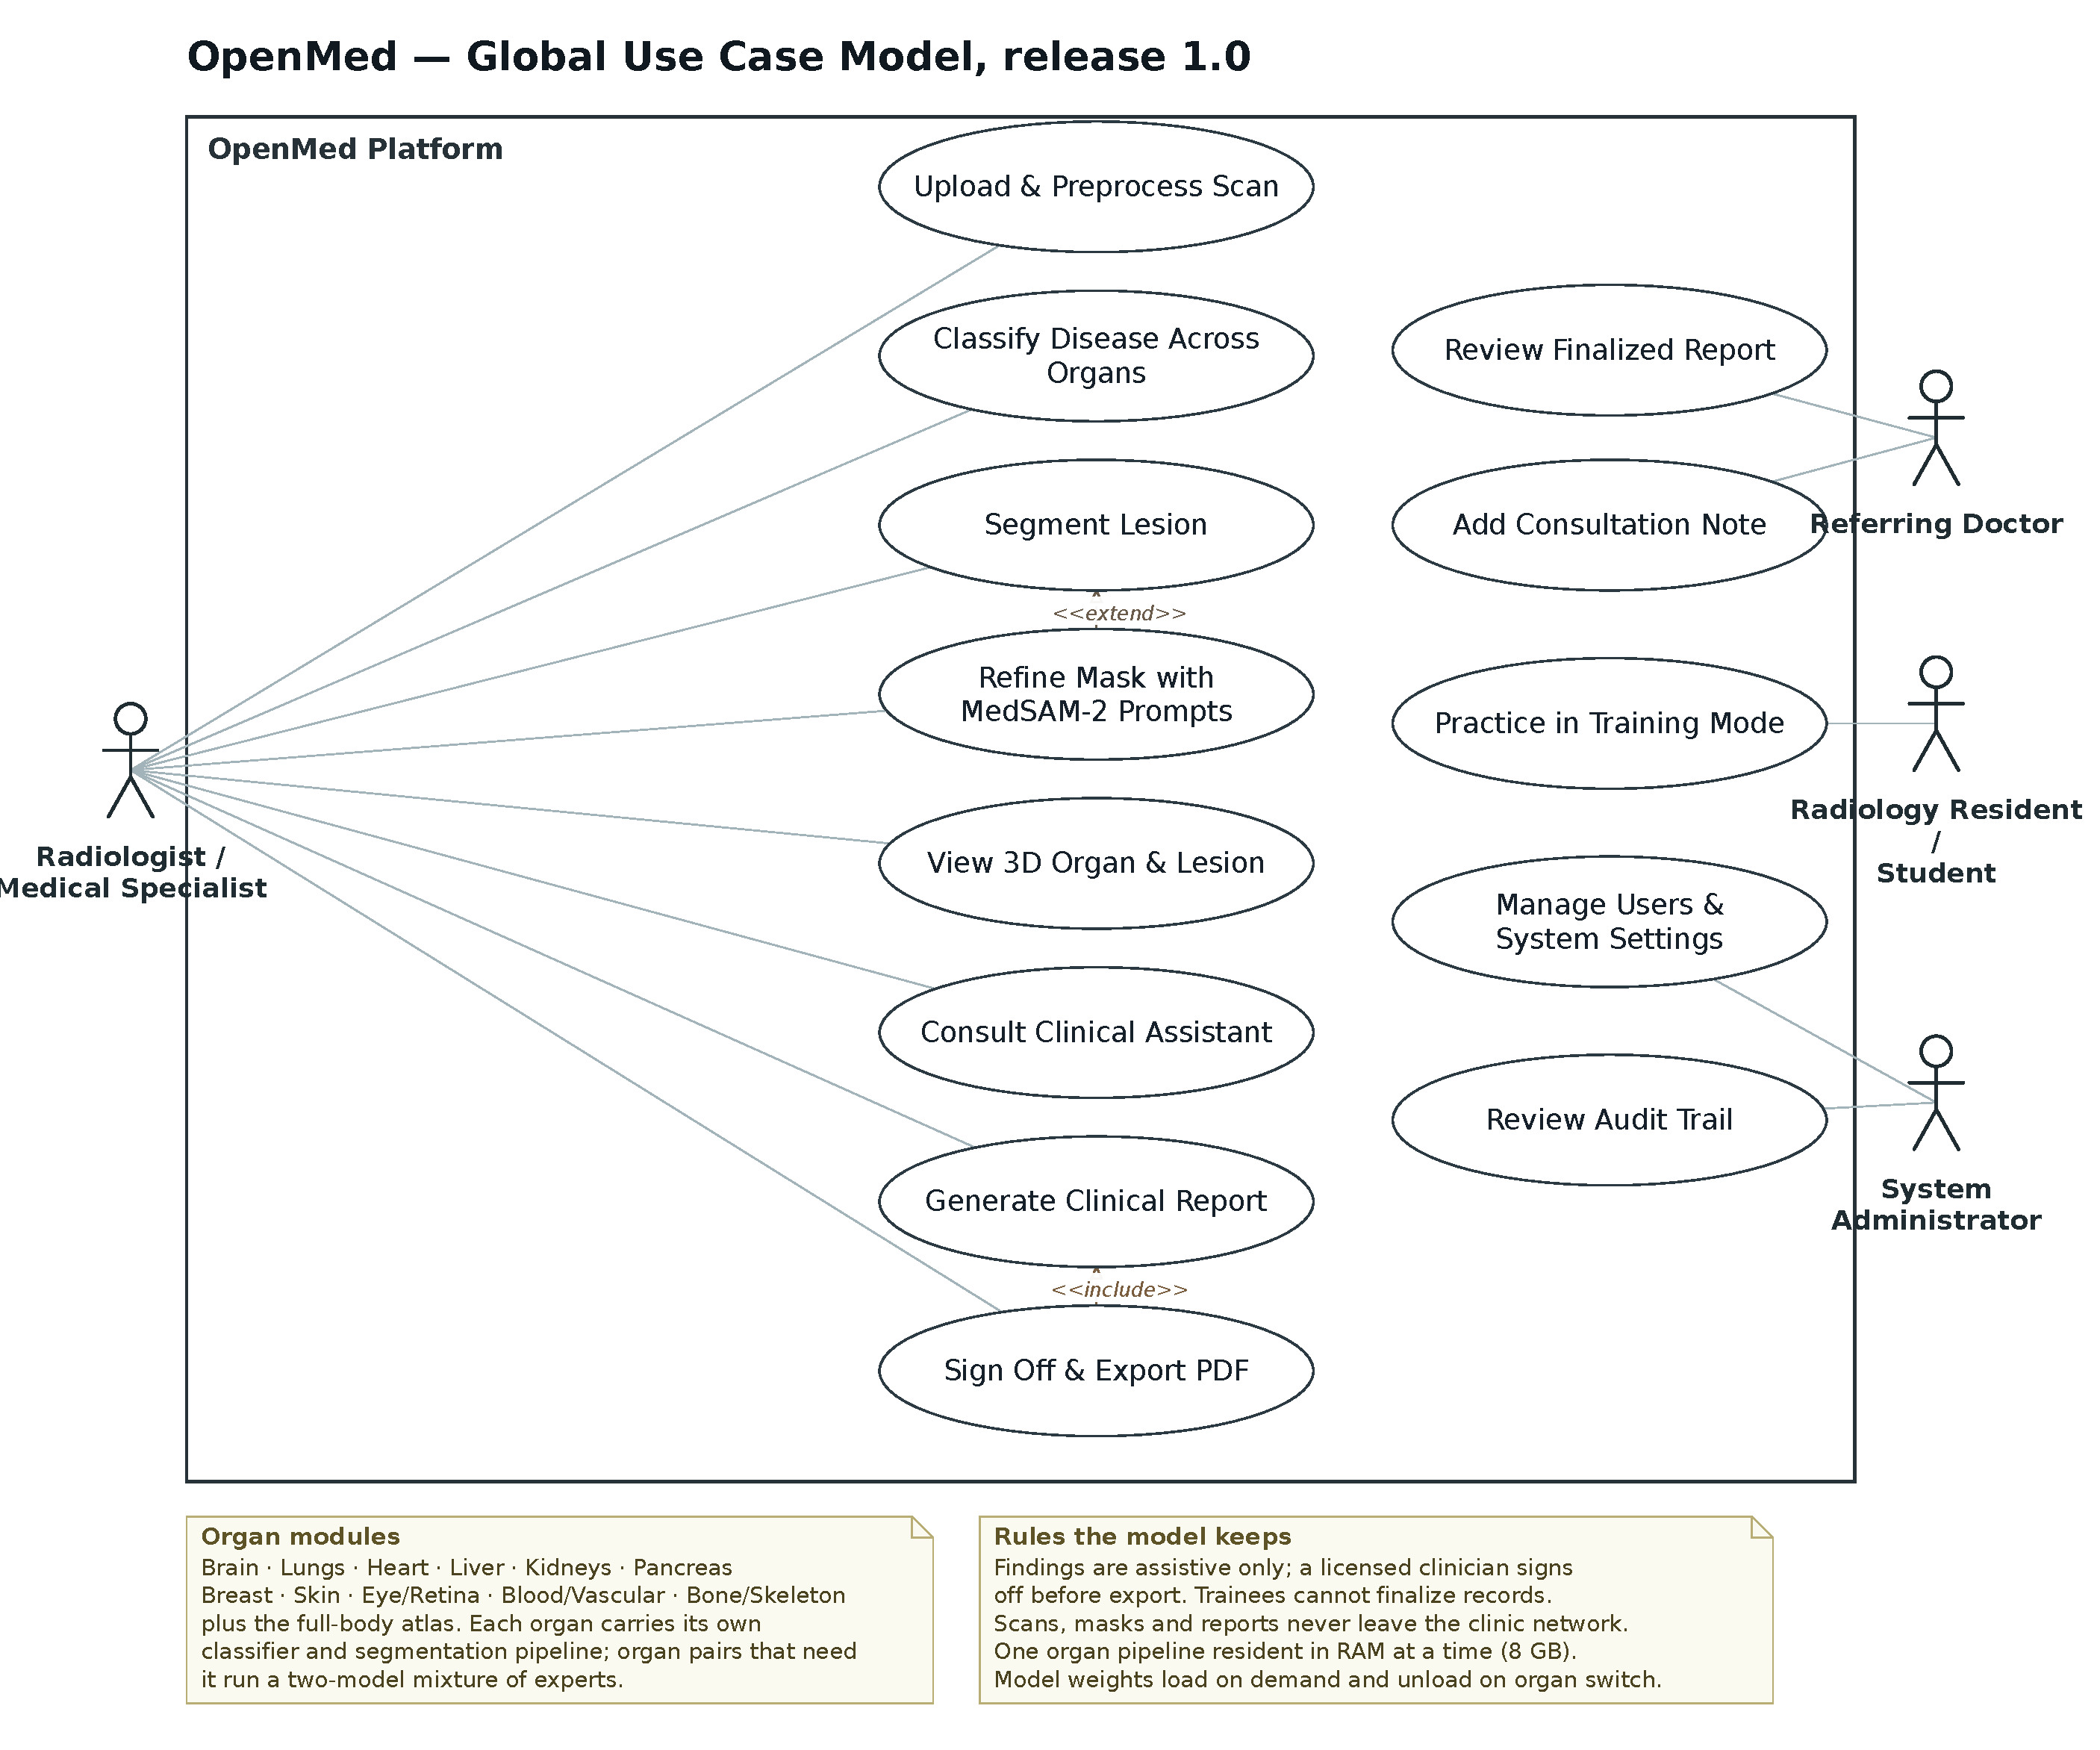
\includegraphics[width=\textwidth]{10_usecase_diagram.pdf}
    \caption{Use Case Diagram for Clinician, Radiologist, Referring Doctor and Administrator}
    \label{fig:usecase_diagram}
\end{figure}

\subsubsection{Entity-Relationship Diagram}
The data model in crow's foot notation. Findings, masks, and reports are versioned rather than overwritten, so a case keeps every intermediate reading it ever produced. Attribute names are taken from the response contracts the routers return, not invented for the diagram.

\begin{figure}[H]
    \centering
    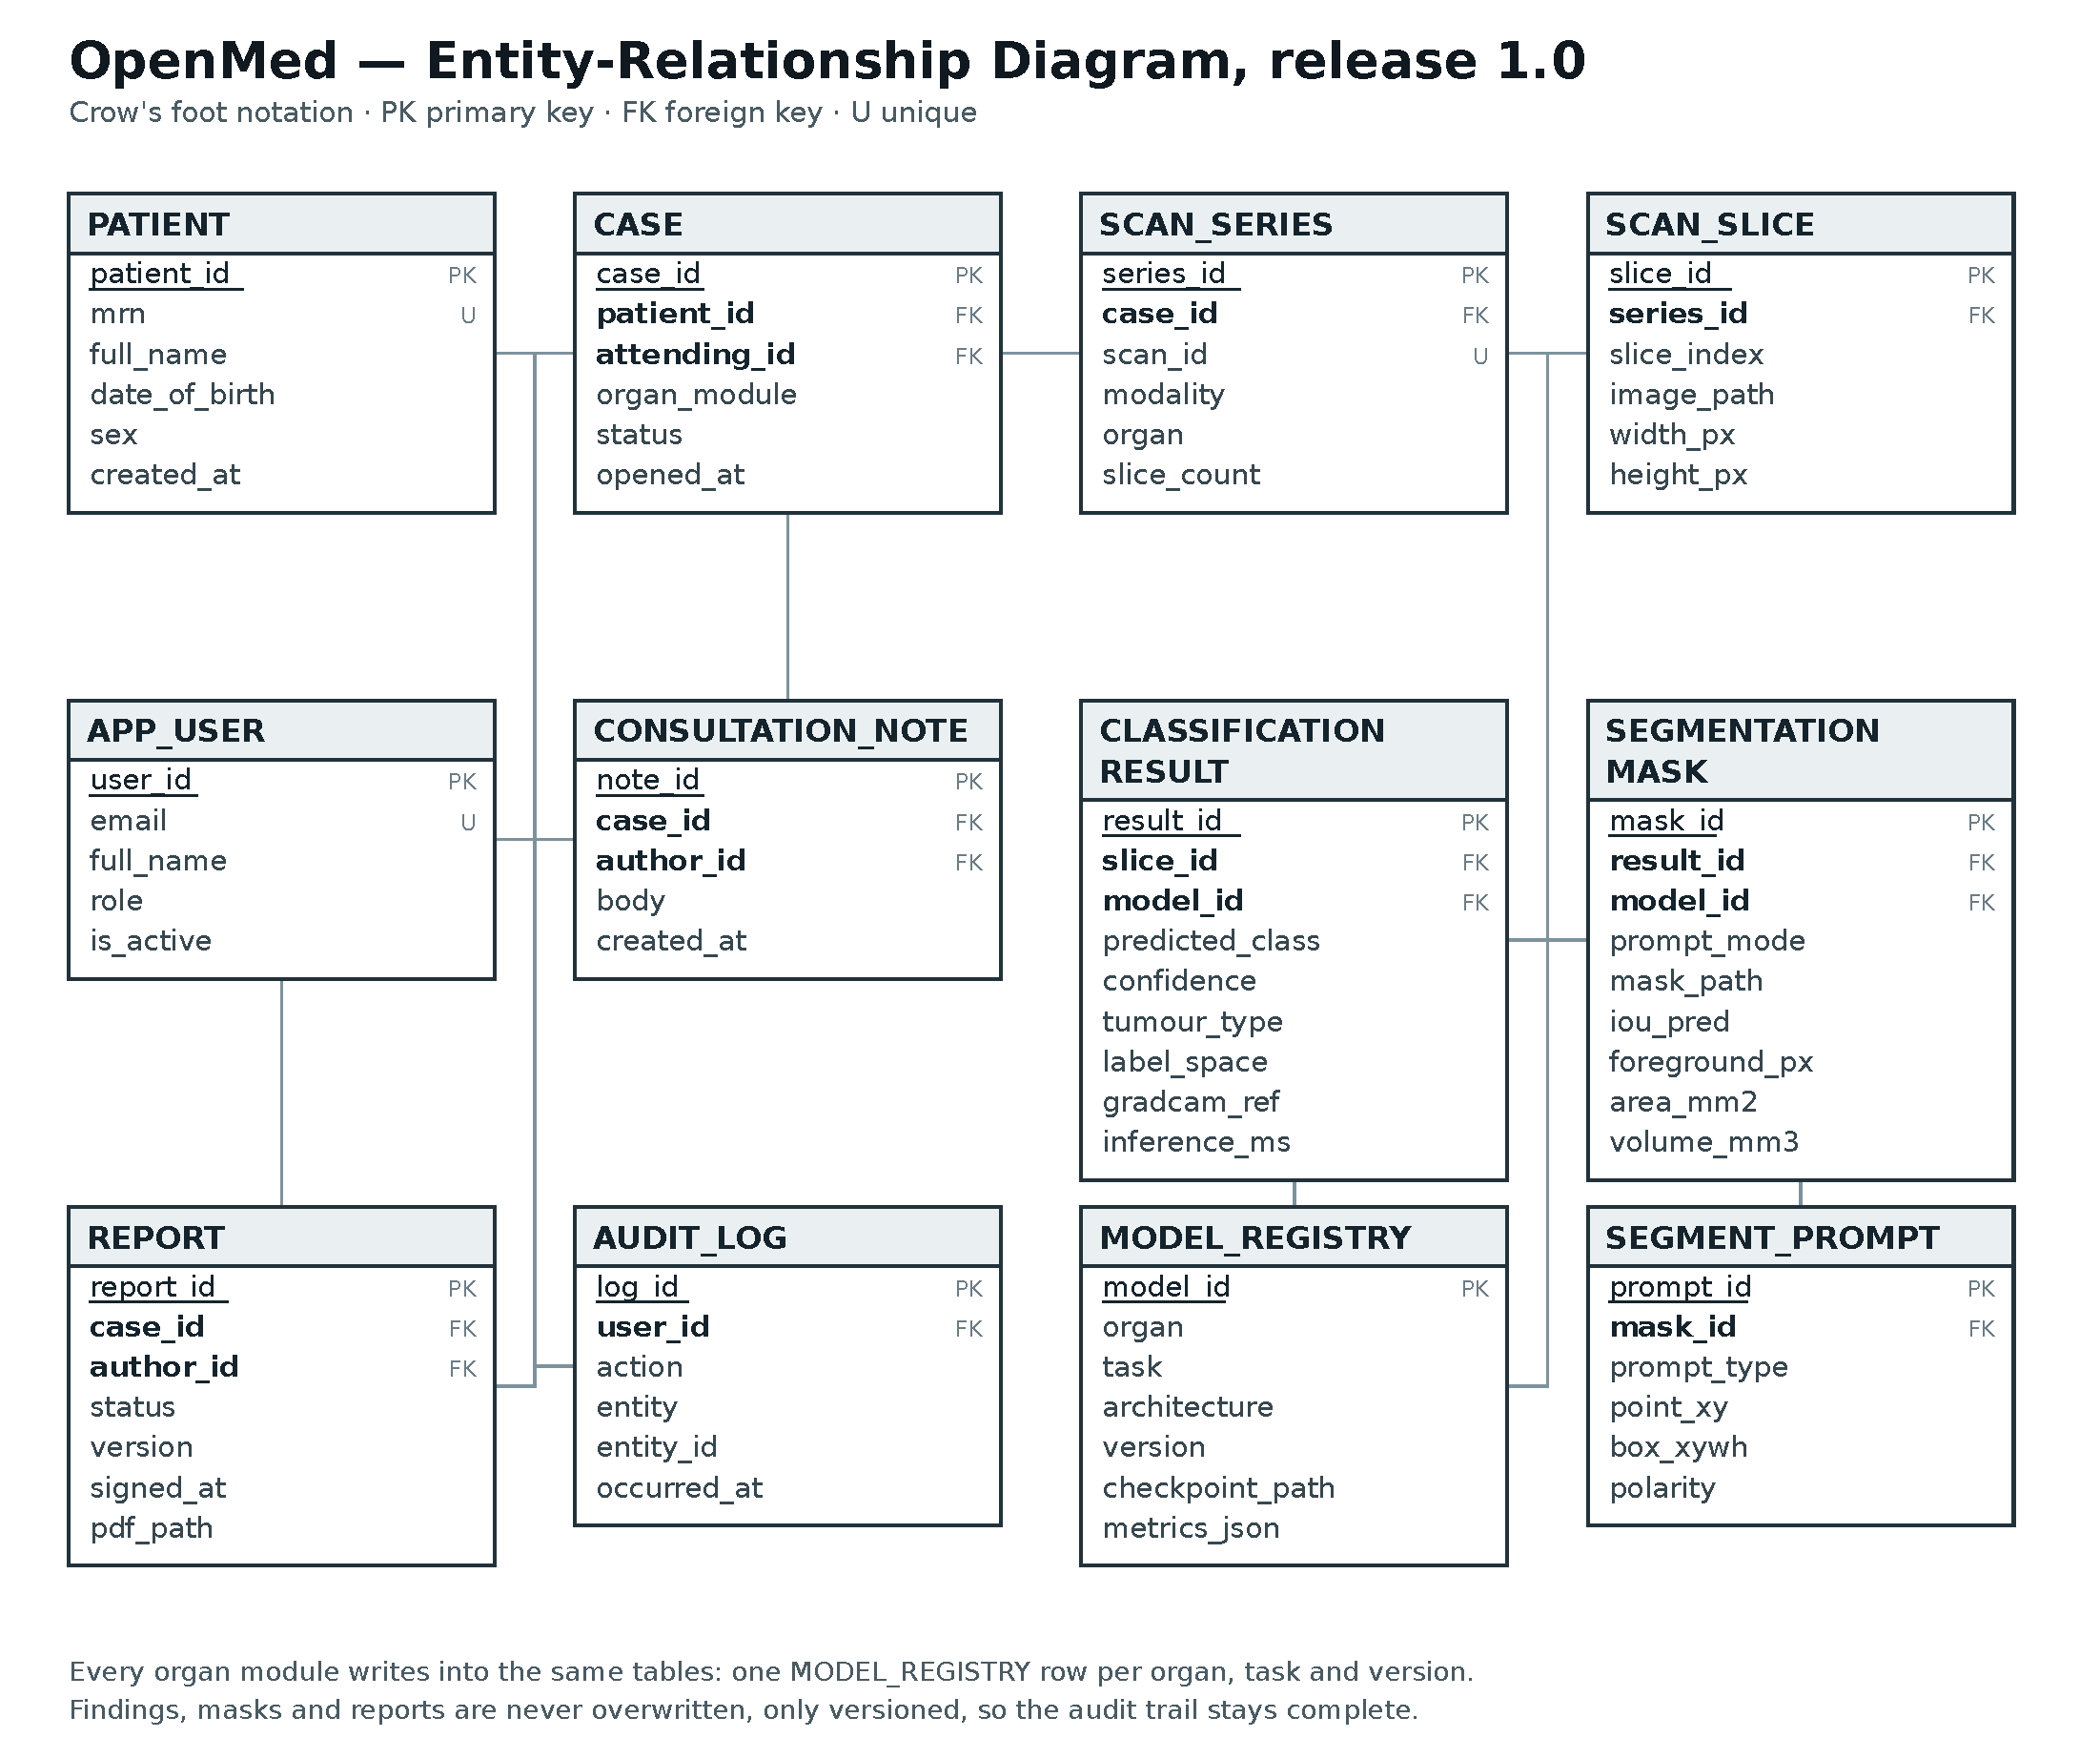
\includegraphics[width=\textwidth]{11_er_diagram.pdf}
    \caption{Entity-Relationship Diagram for Patient, Case, Series, Result, Mask and Report}
    \label{fig:er_diagram}
\end{figure}

\subsubsection{Architectural Diagram}
The deployment view: React and TypeScript in the browser, a FastAPI service, one inference engine per organ task, and the MedSAM-2 pipeline reached over a WebSocket. Nothing crosses the clinic boundary, which is Rule 3 of the business rules.

\begin{figure}[H]
    \centering
    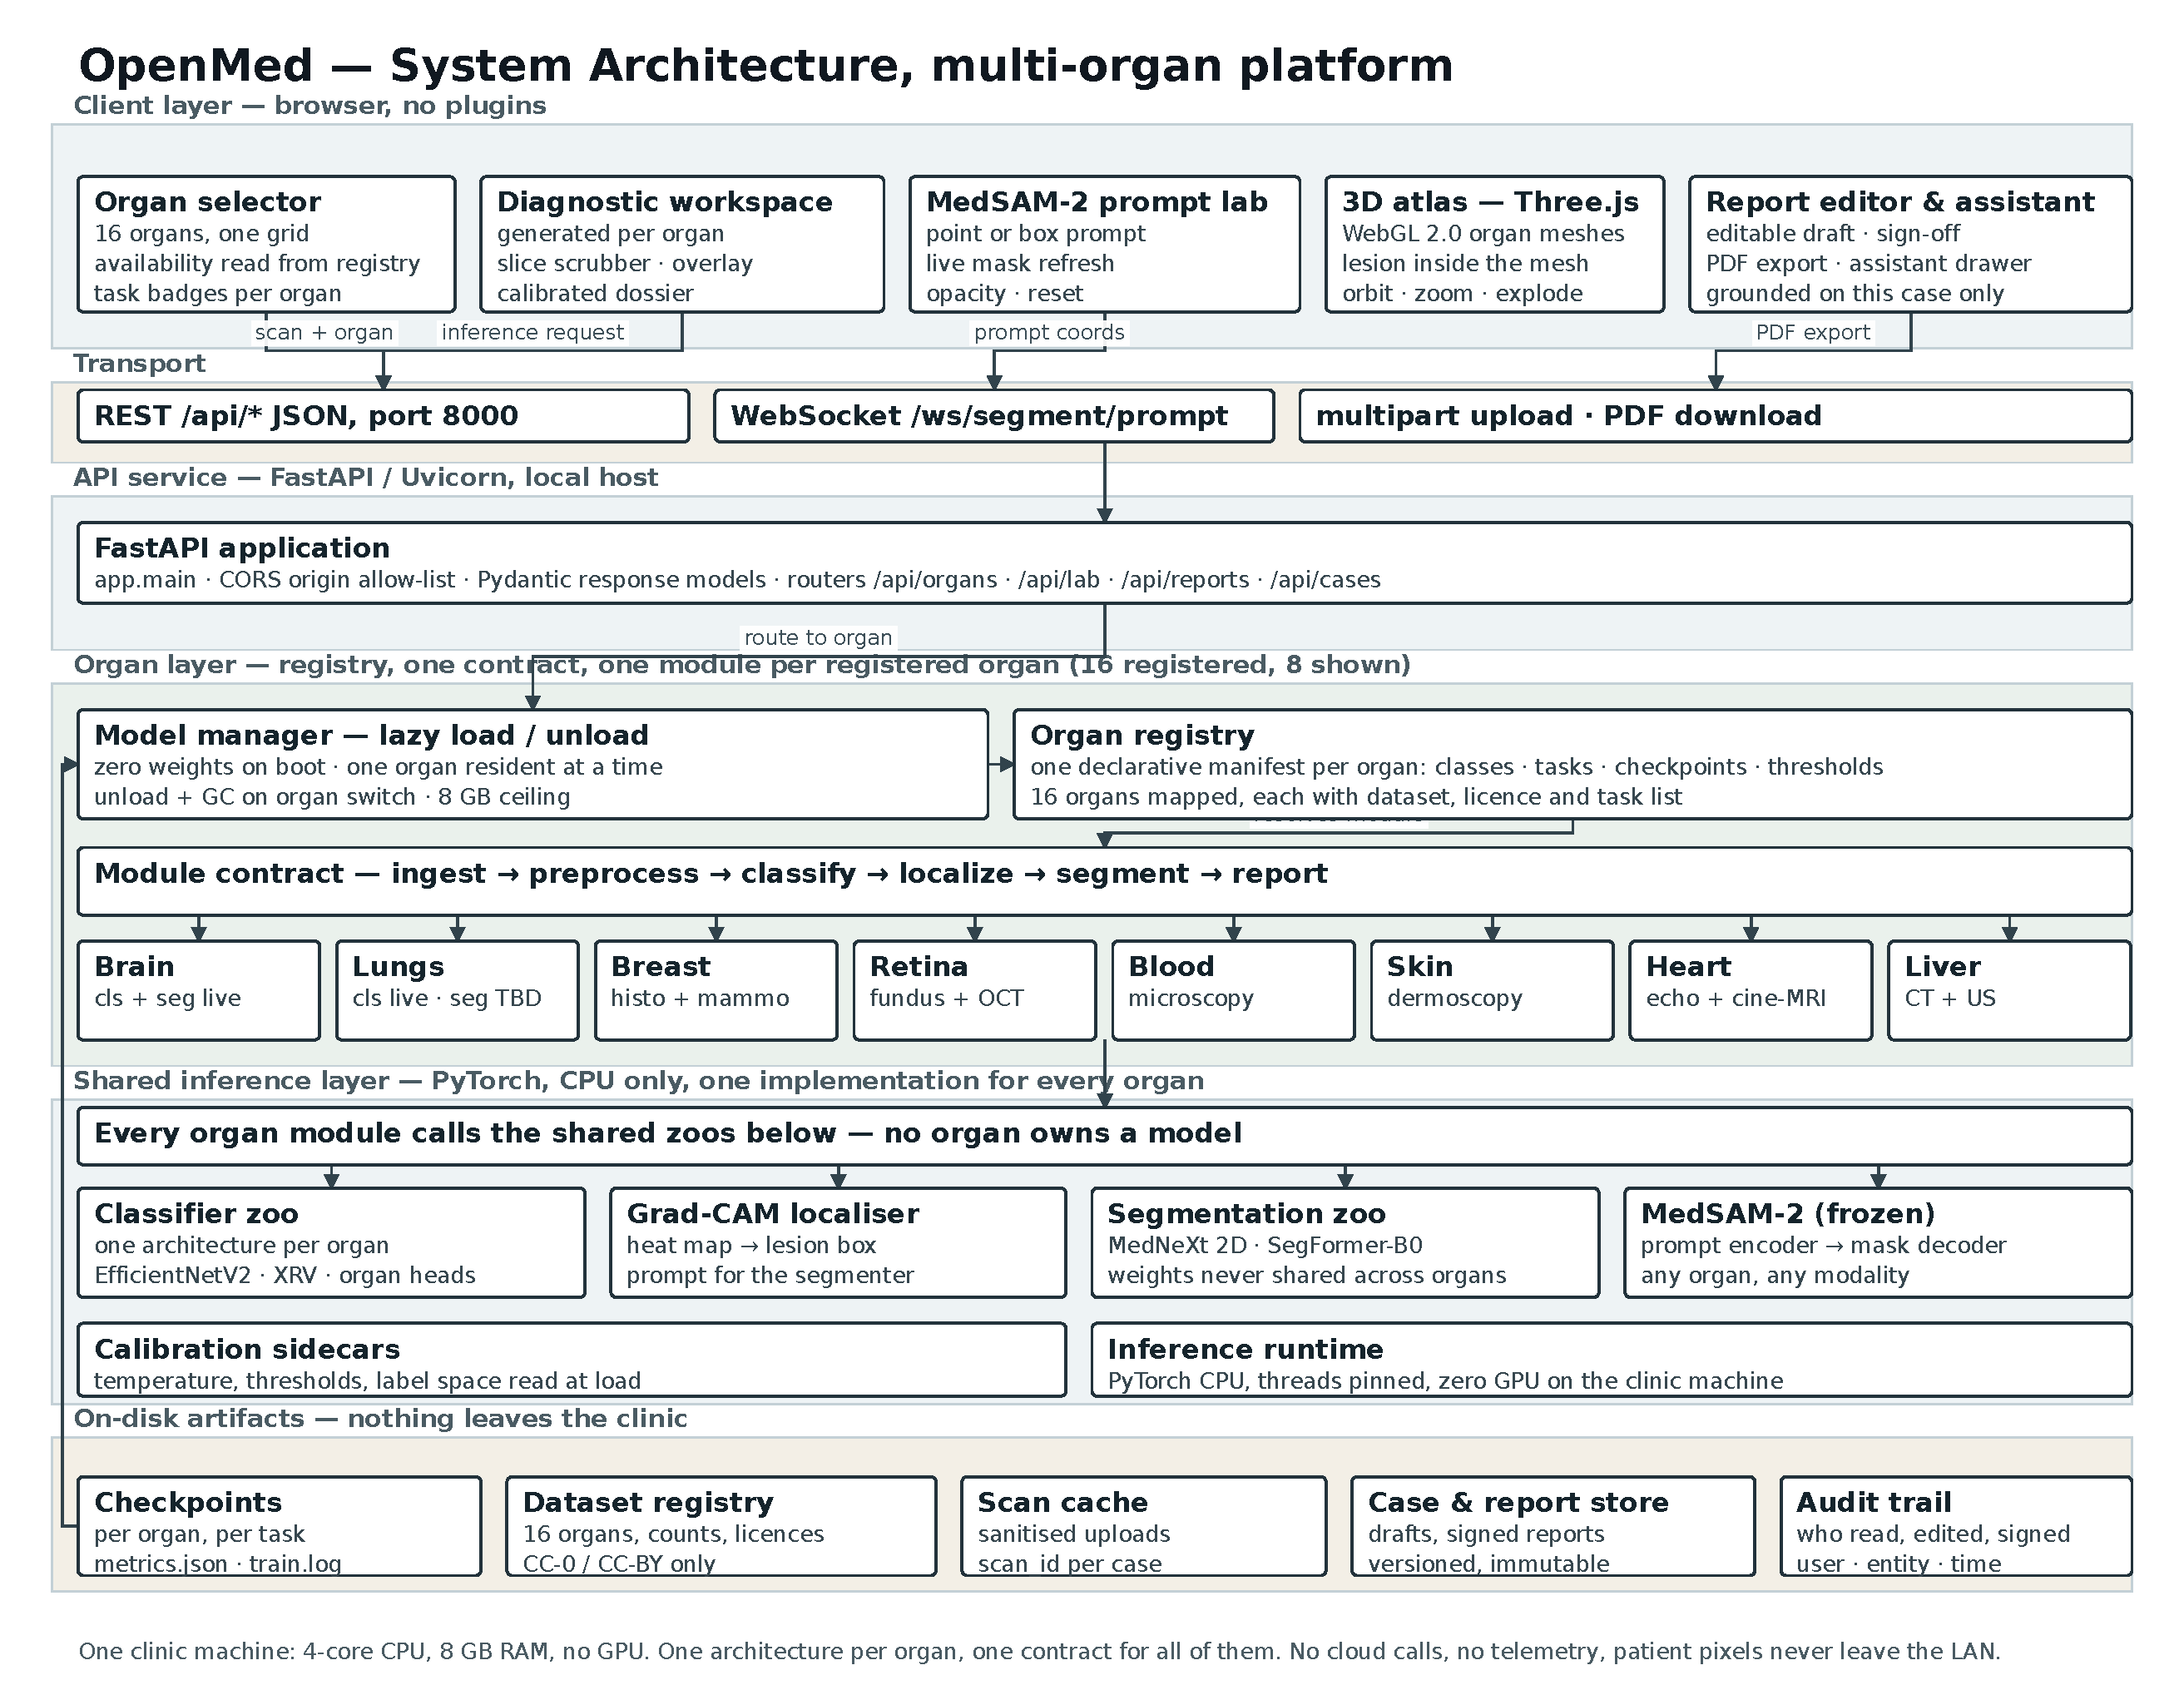
\includegraphics[width=\textwidth]{12_architecture_diagram.pdf}
    \caption{System Architecture with Backend Inference Engines and WebGL Client}
    \label{fig:architecture_diagram}
\end{figure}

\subsubsection{Activity Diagram}
One case from upload to exported PDF. The decision points are the ones the code actually takes: whether the scan validates, whether the classification is Normal, whether the clinician asks for a refinement, and whether the report is signed.

\begin{figure}[H]
    \centering
    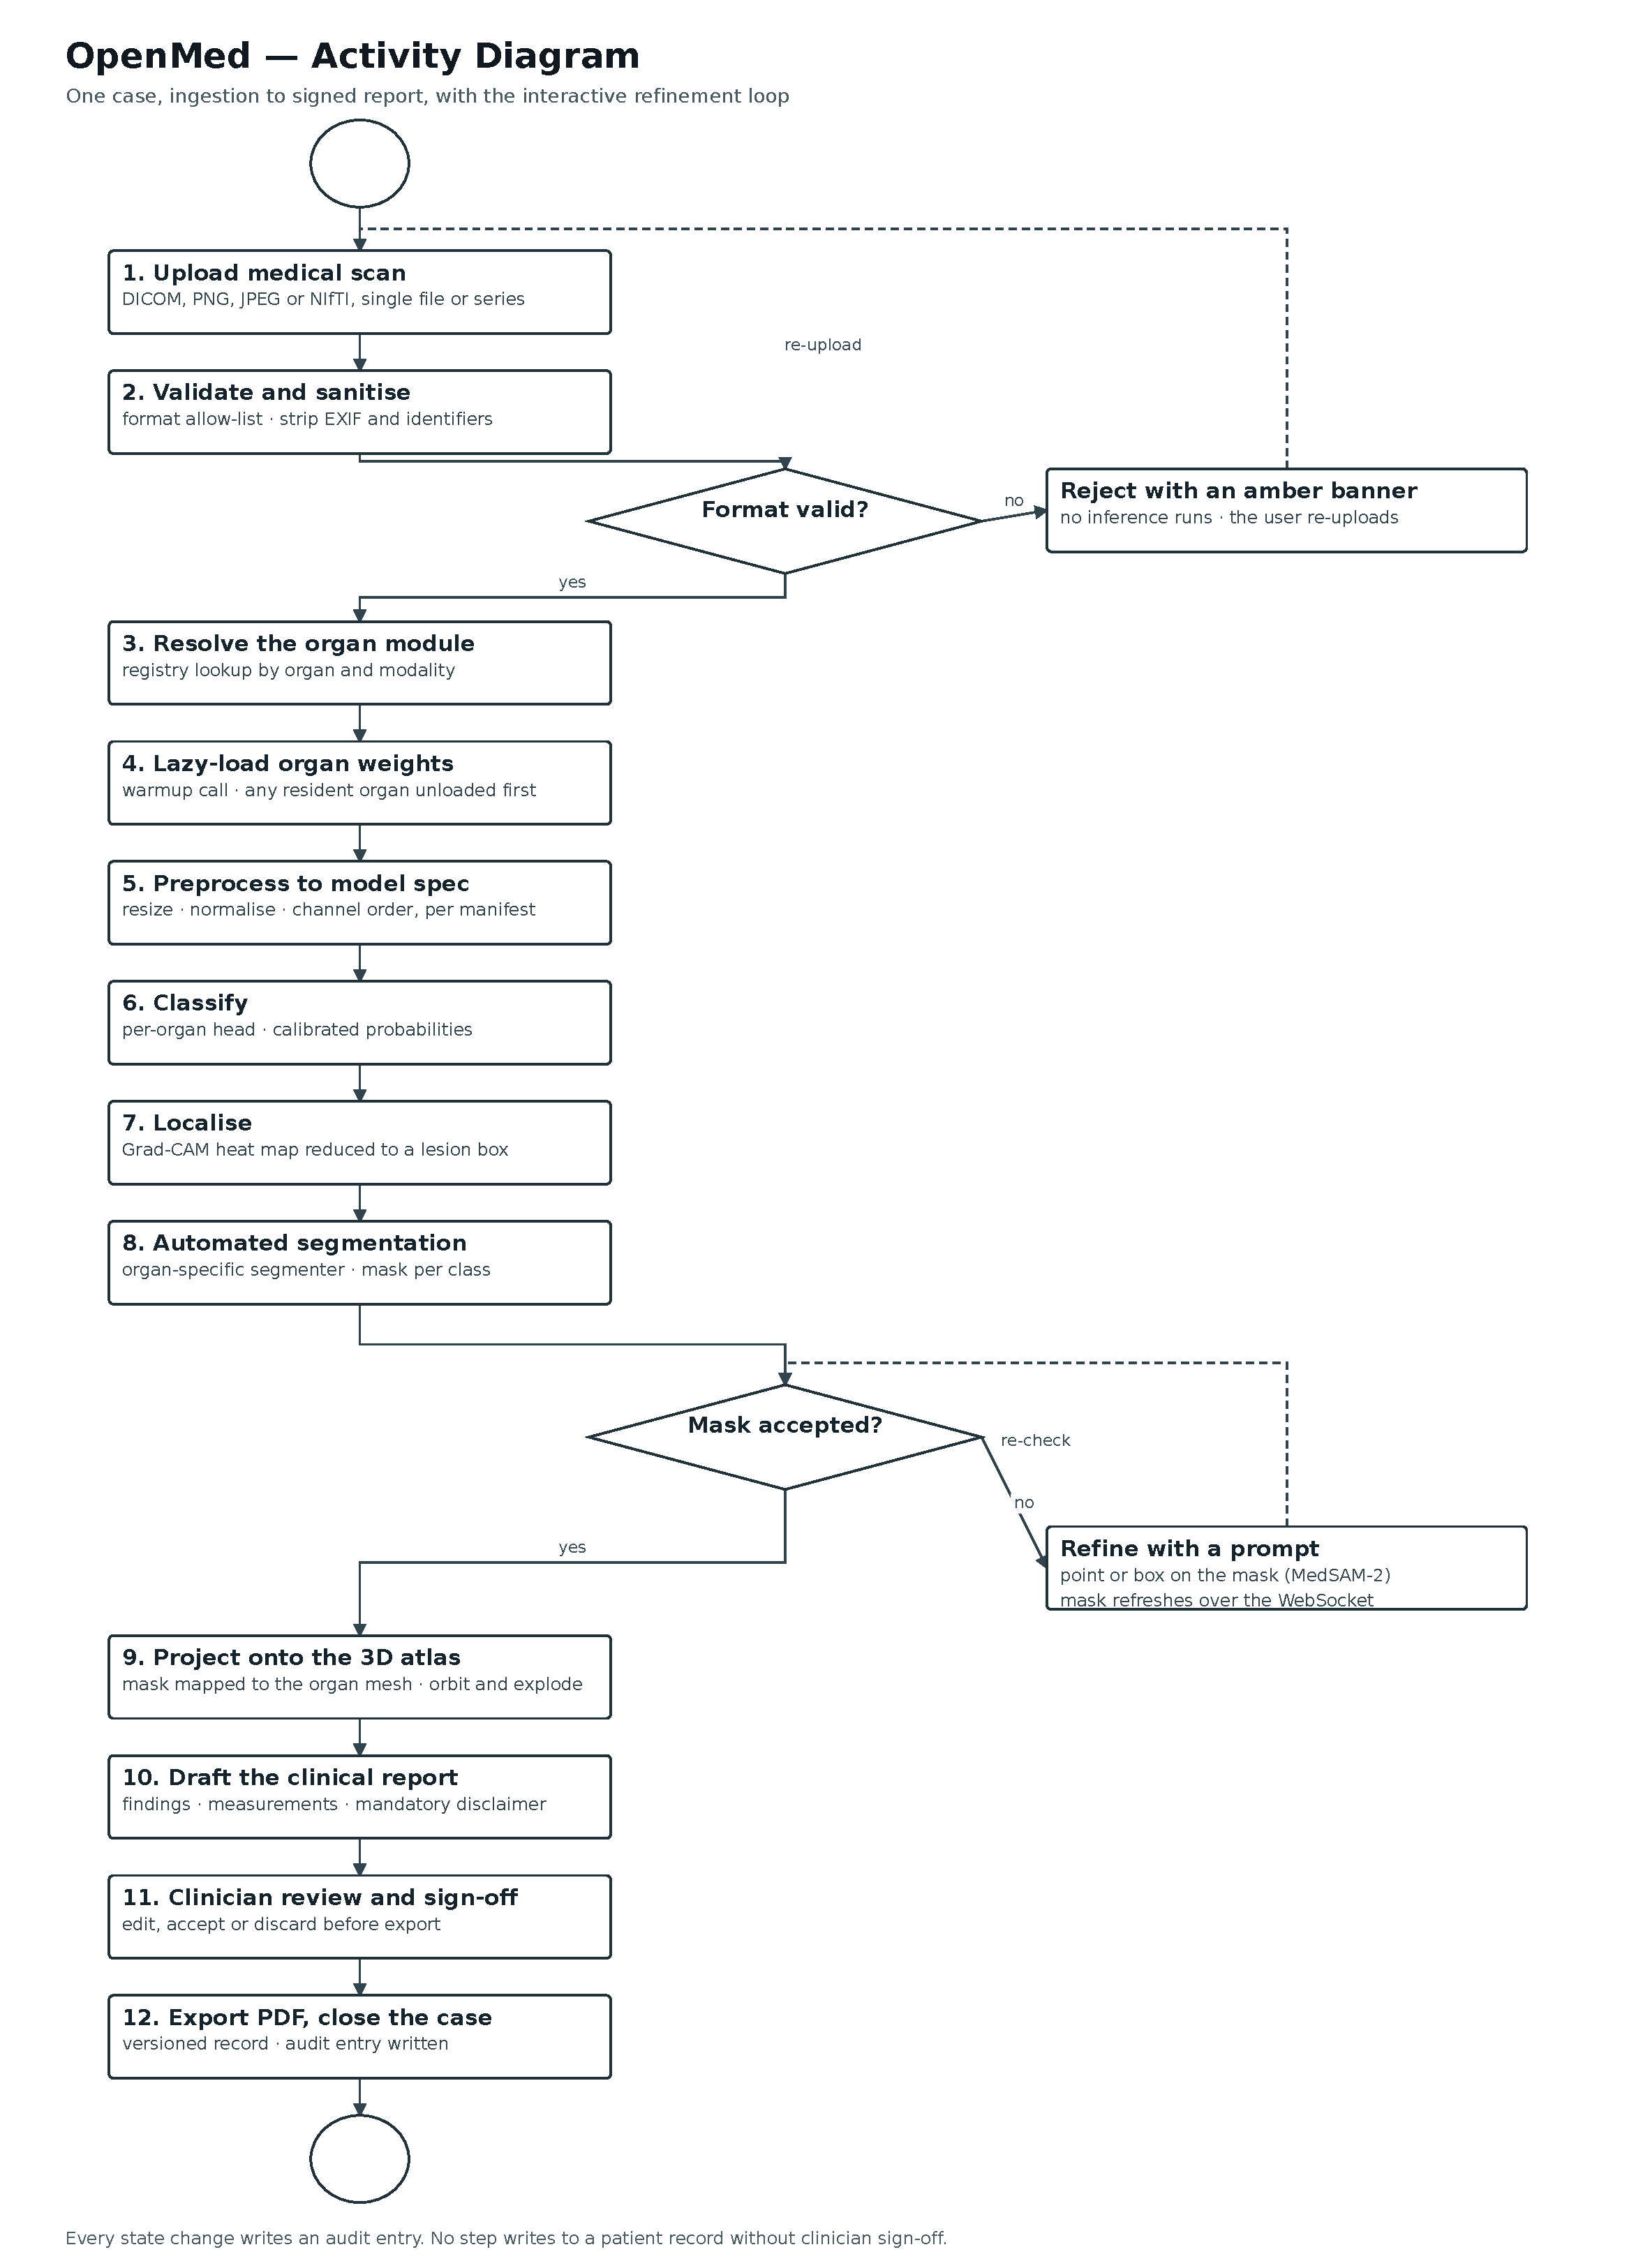
\includegraphics[width=\textwidth]{13_activity_diagram.pdf}
    \caption{Activity Diagram from Scan Ingestion to Interactive Refinement and PDF Export}
    \label{fig:activity_diagram}
\end{figure}

\subsubsection{Sequence Diagram}
The message order for a single case across six participants. Dashed arrows are returns. The refinement loop is the only part that is not request and response: the browser keeps a socket open and the mask comes back as an update rather than as a new document.

\begin{figure}[H]
    \centering
    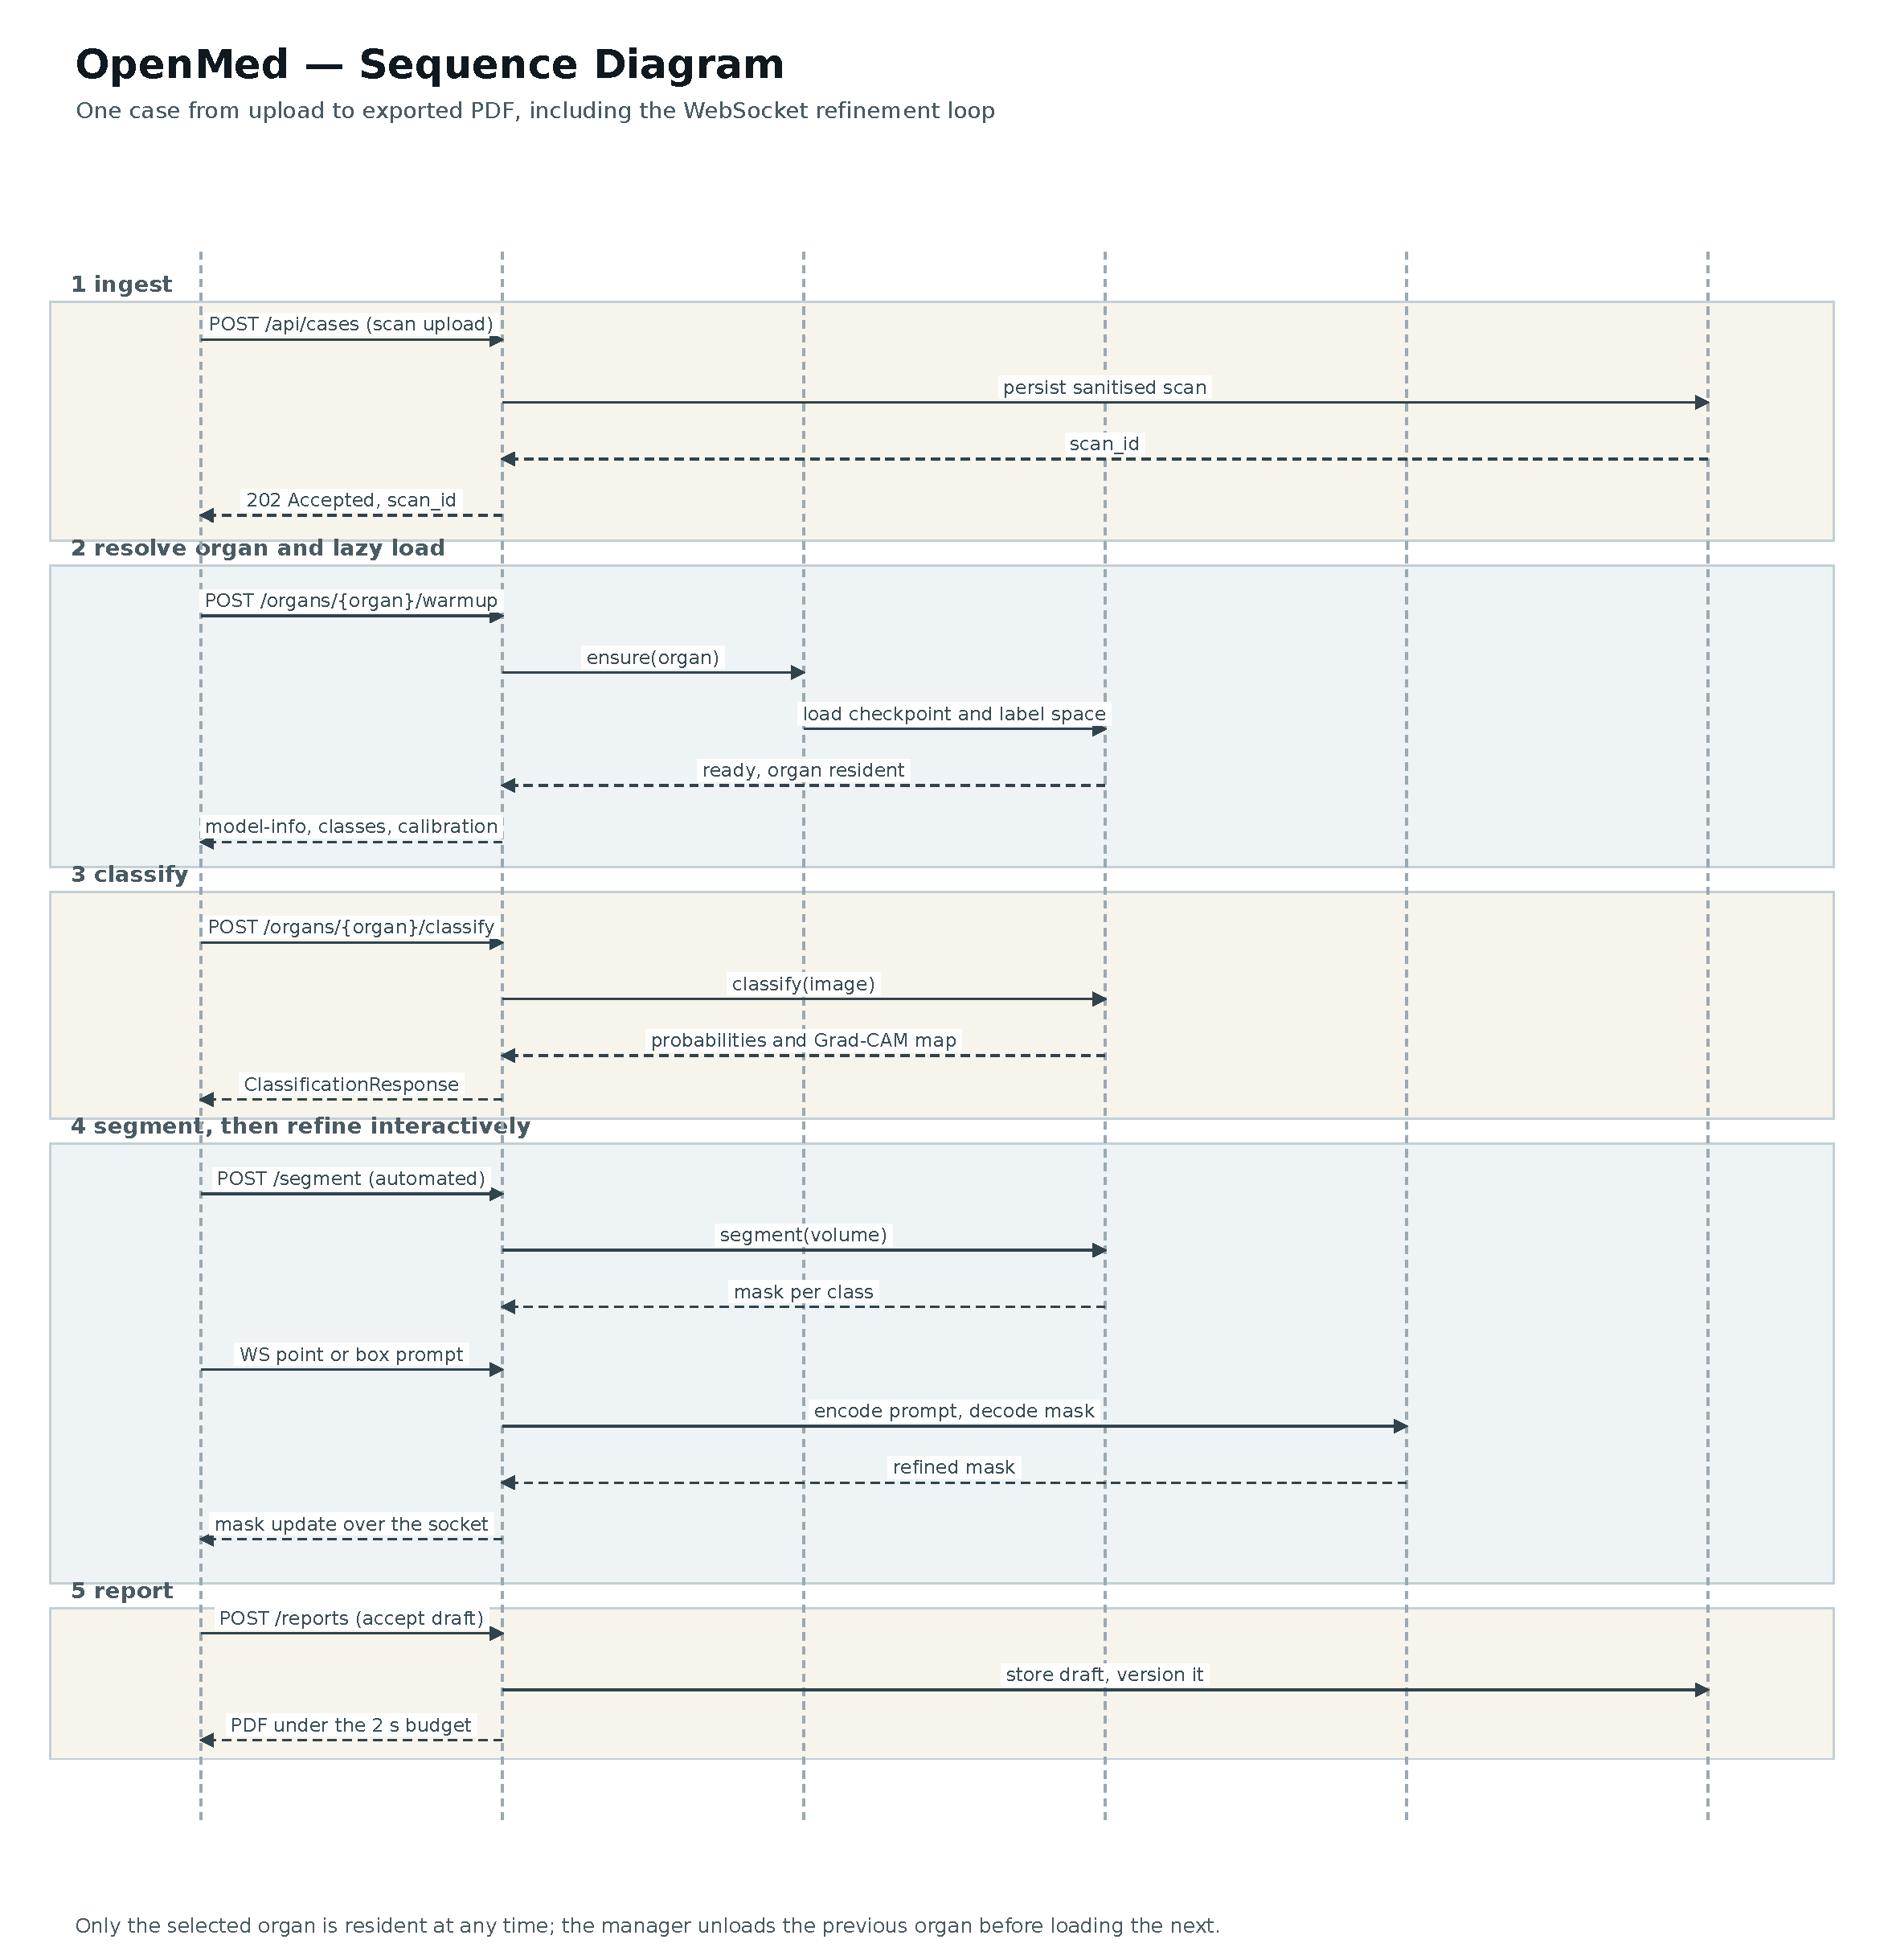
\includegraphics[width=\textwidth]{14_sequence_diagram.pdf}
    \caption{Sequence Diagram for Ingestion, Lazy Organ Load, Inference and WebSocket Refinement}
    \label{fig:sequence_diagram}
\end{figure}

\subsubsection{Component Diagram}
Five tiers, and the domain tier instantiates one module per registered organ. Adapters are shared code; weights and configuration are not. Each organ module owns its own checkpoint and manifest, and the calibration sidecar reads its temperature from the manifest beside that checkpoint.

\begin{figure}[H]
    \centering
    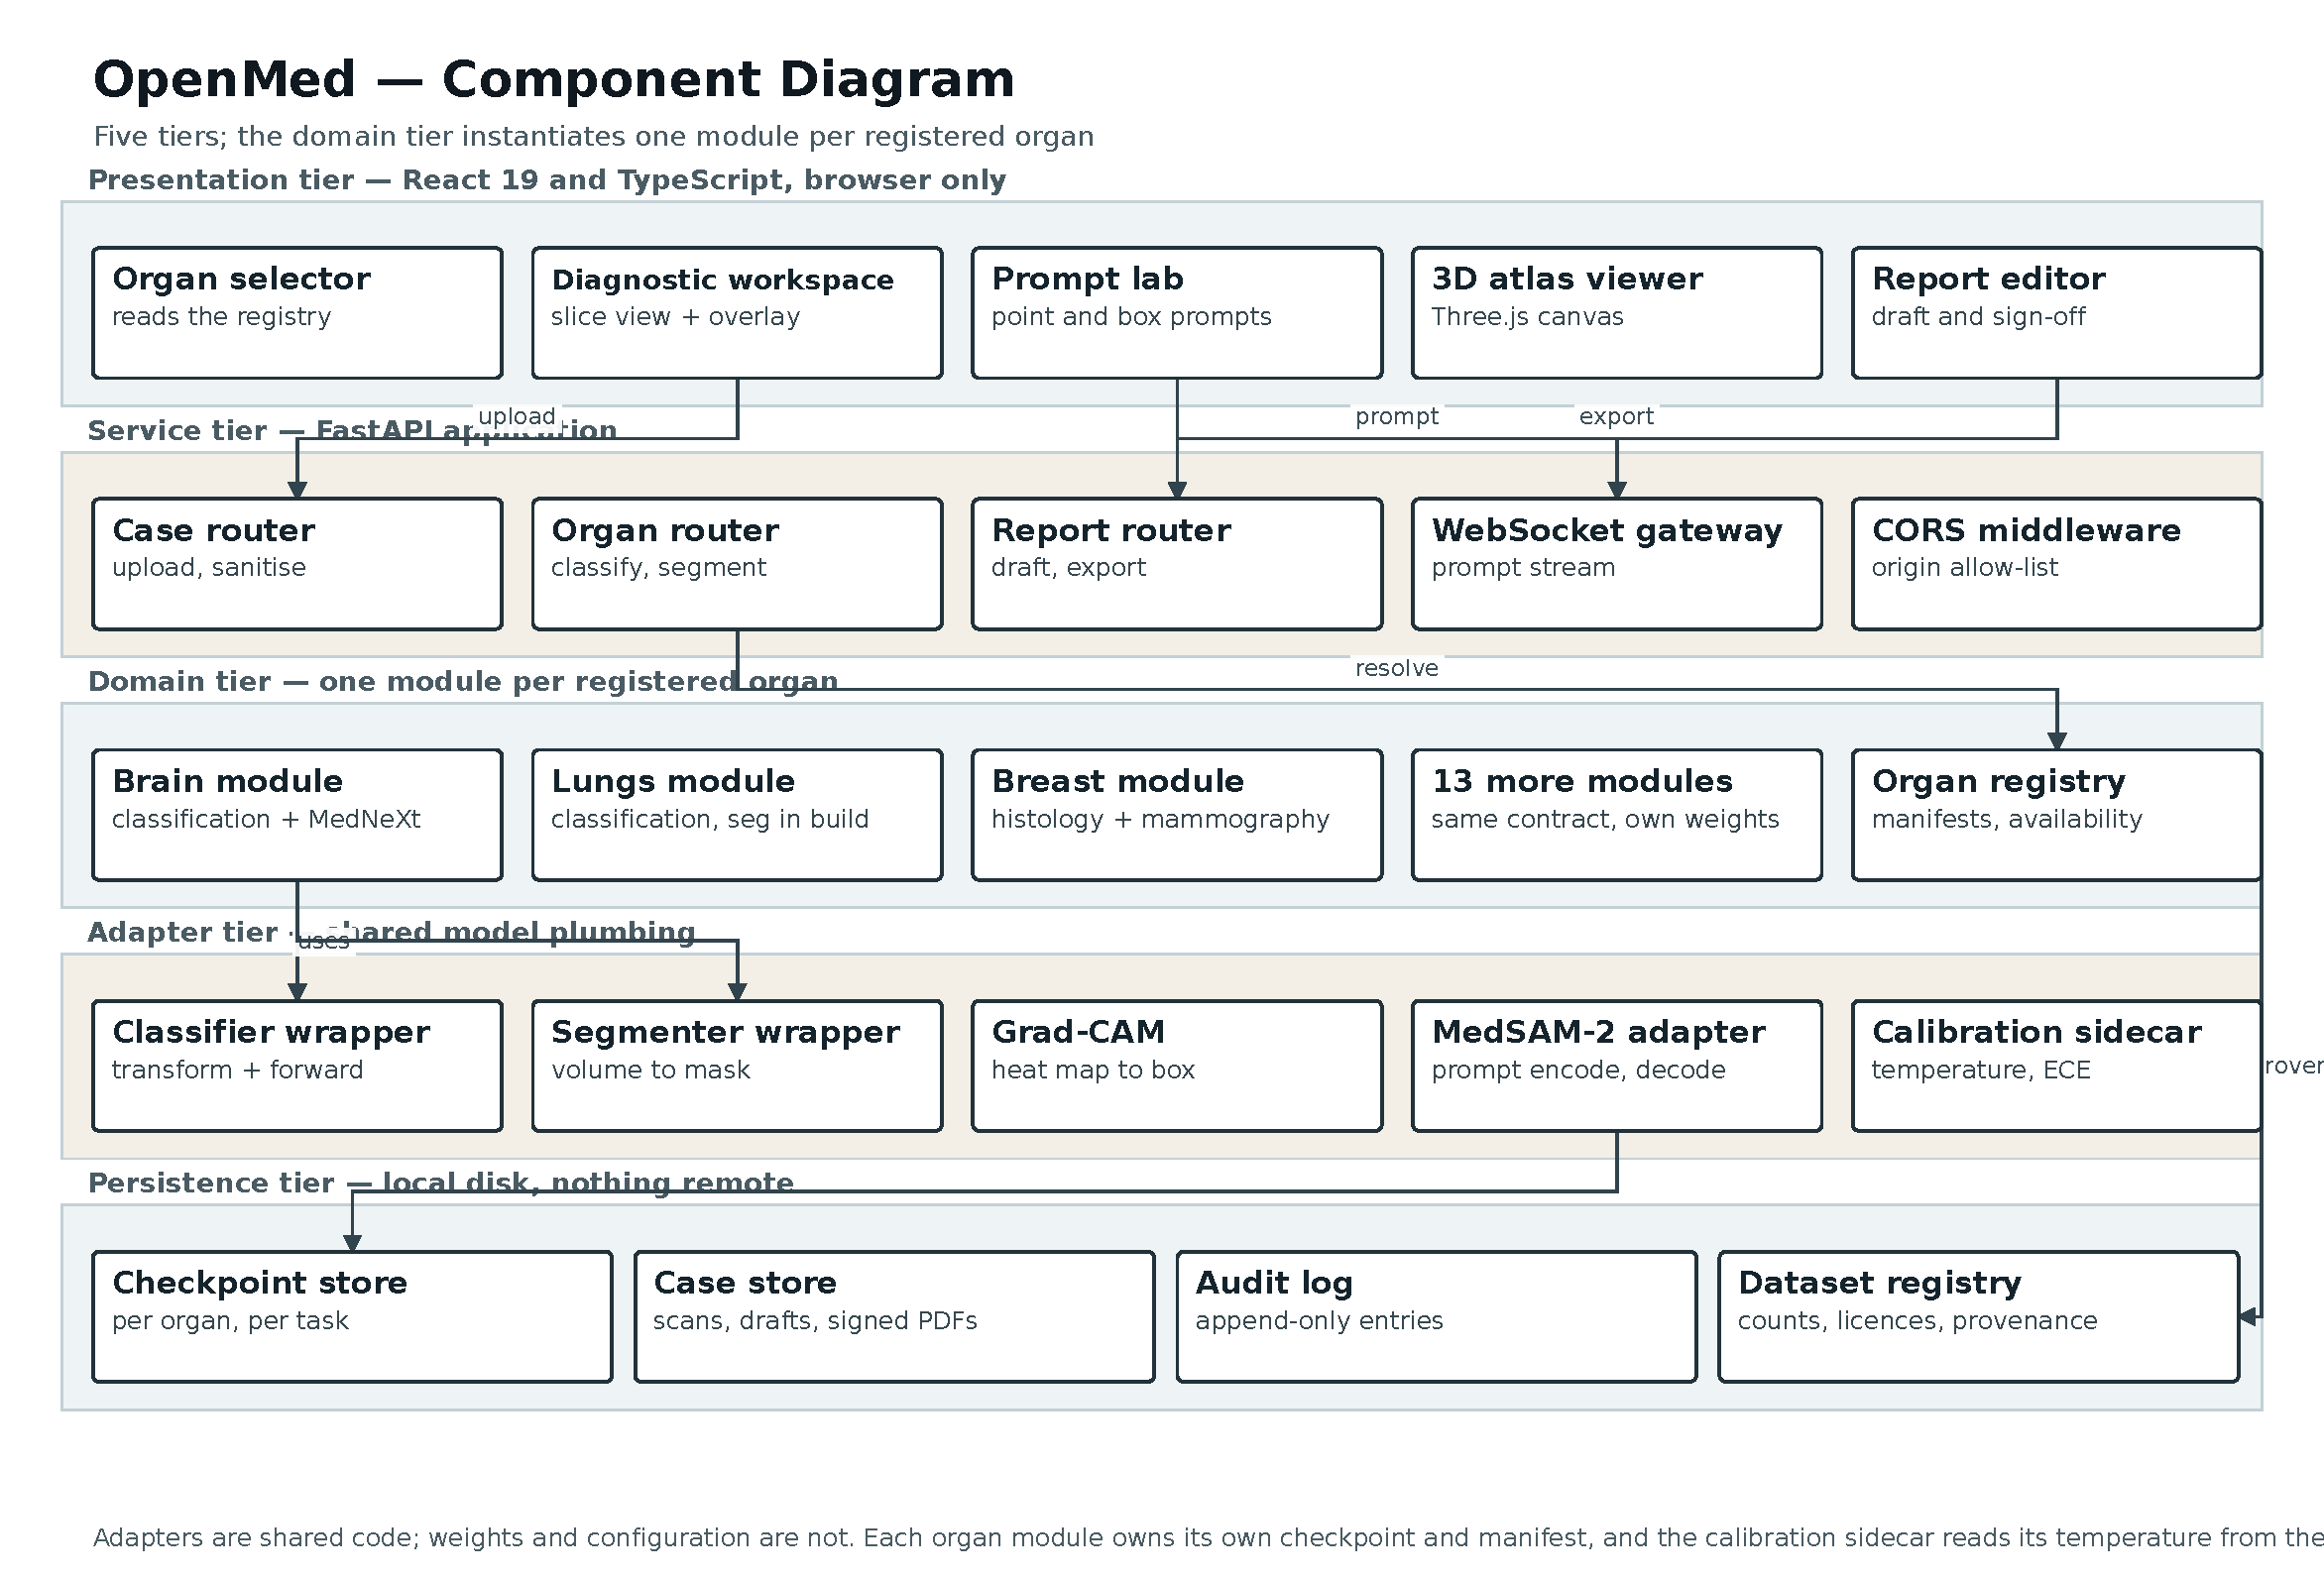
\includegraphics[width=\textwidth]{15_component_diagram.pdf}
    \caption{Component Diagram of the Presentation, Service, Domain, Adapter and Persistence Tiers}
    \label{fig:component_diagram}
\end{figure}

\subsubsection{State Machine Diagram}
The organ lifecycle that enforces Rule 4. A transition that raises leaves the organ in Unavailable instead of half-loaded, because the pipeline drops its partial state before the exception reaches the router. Health reports the resident set size, so an unload can be shown to have actually returned memory rather than merely dropped a reference.

\begin{figure}[H]
    \centering
    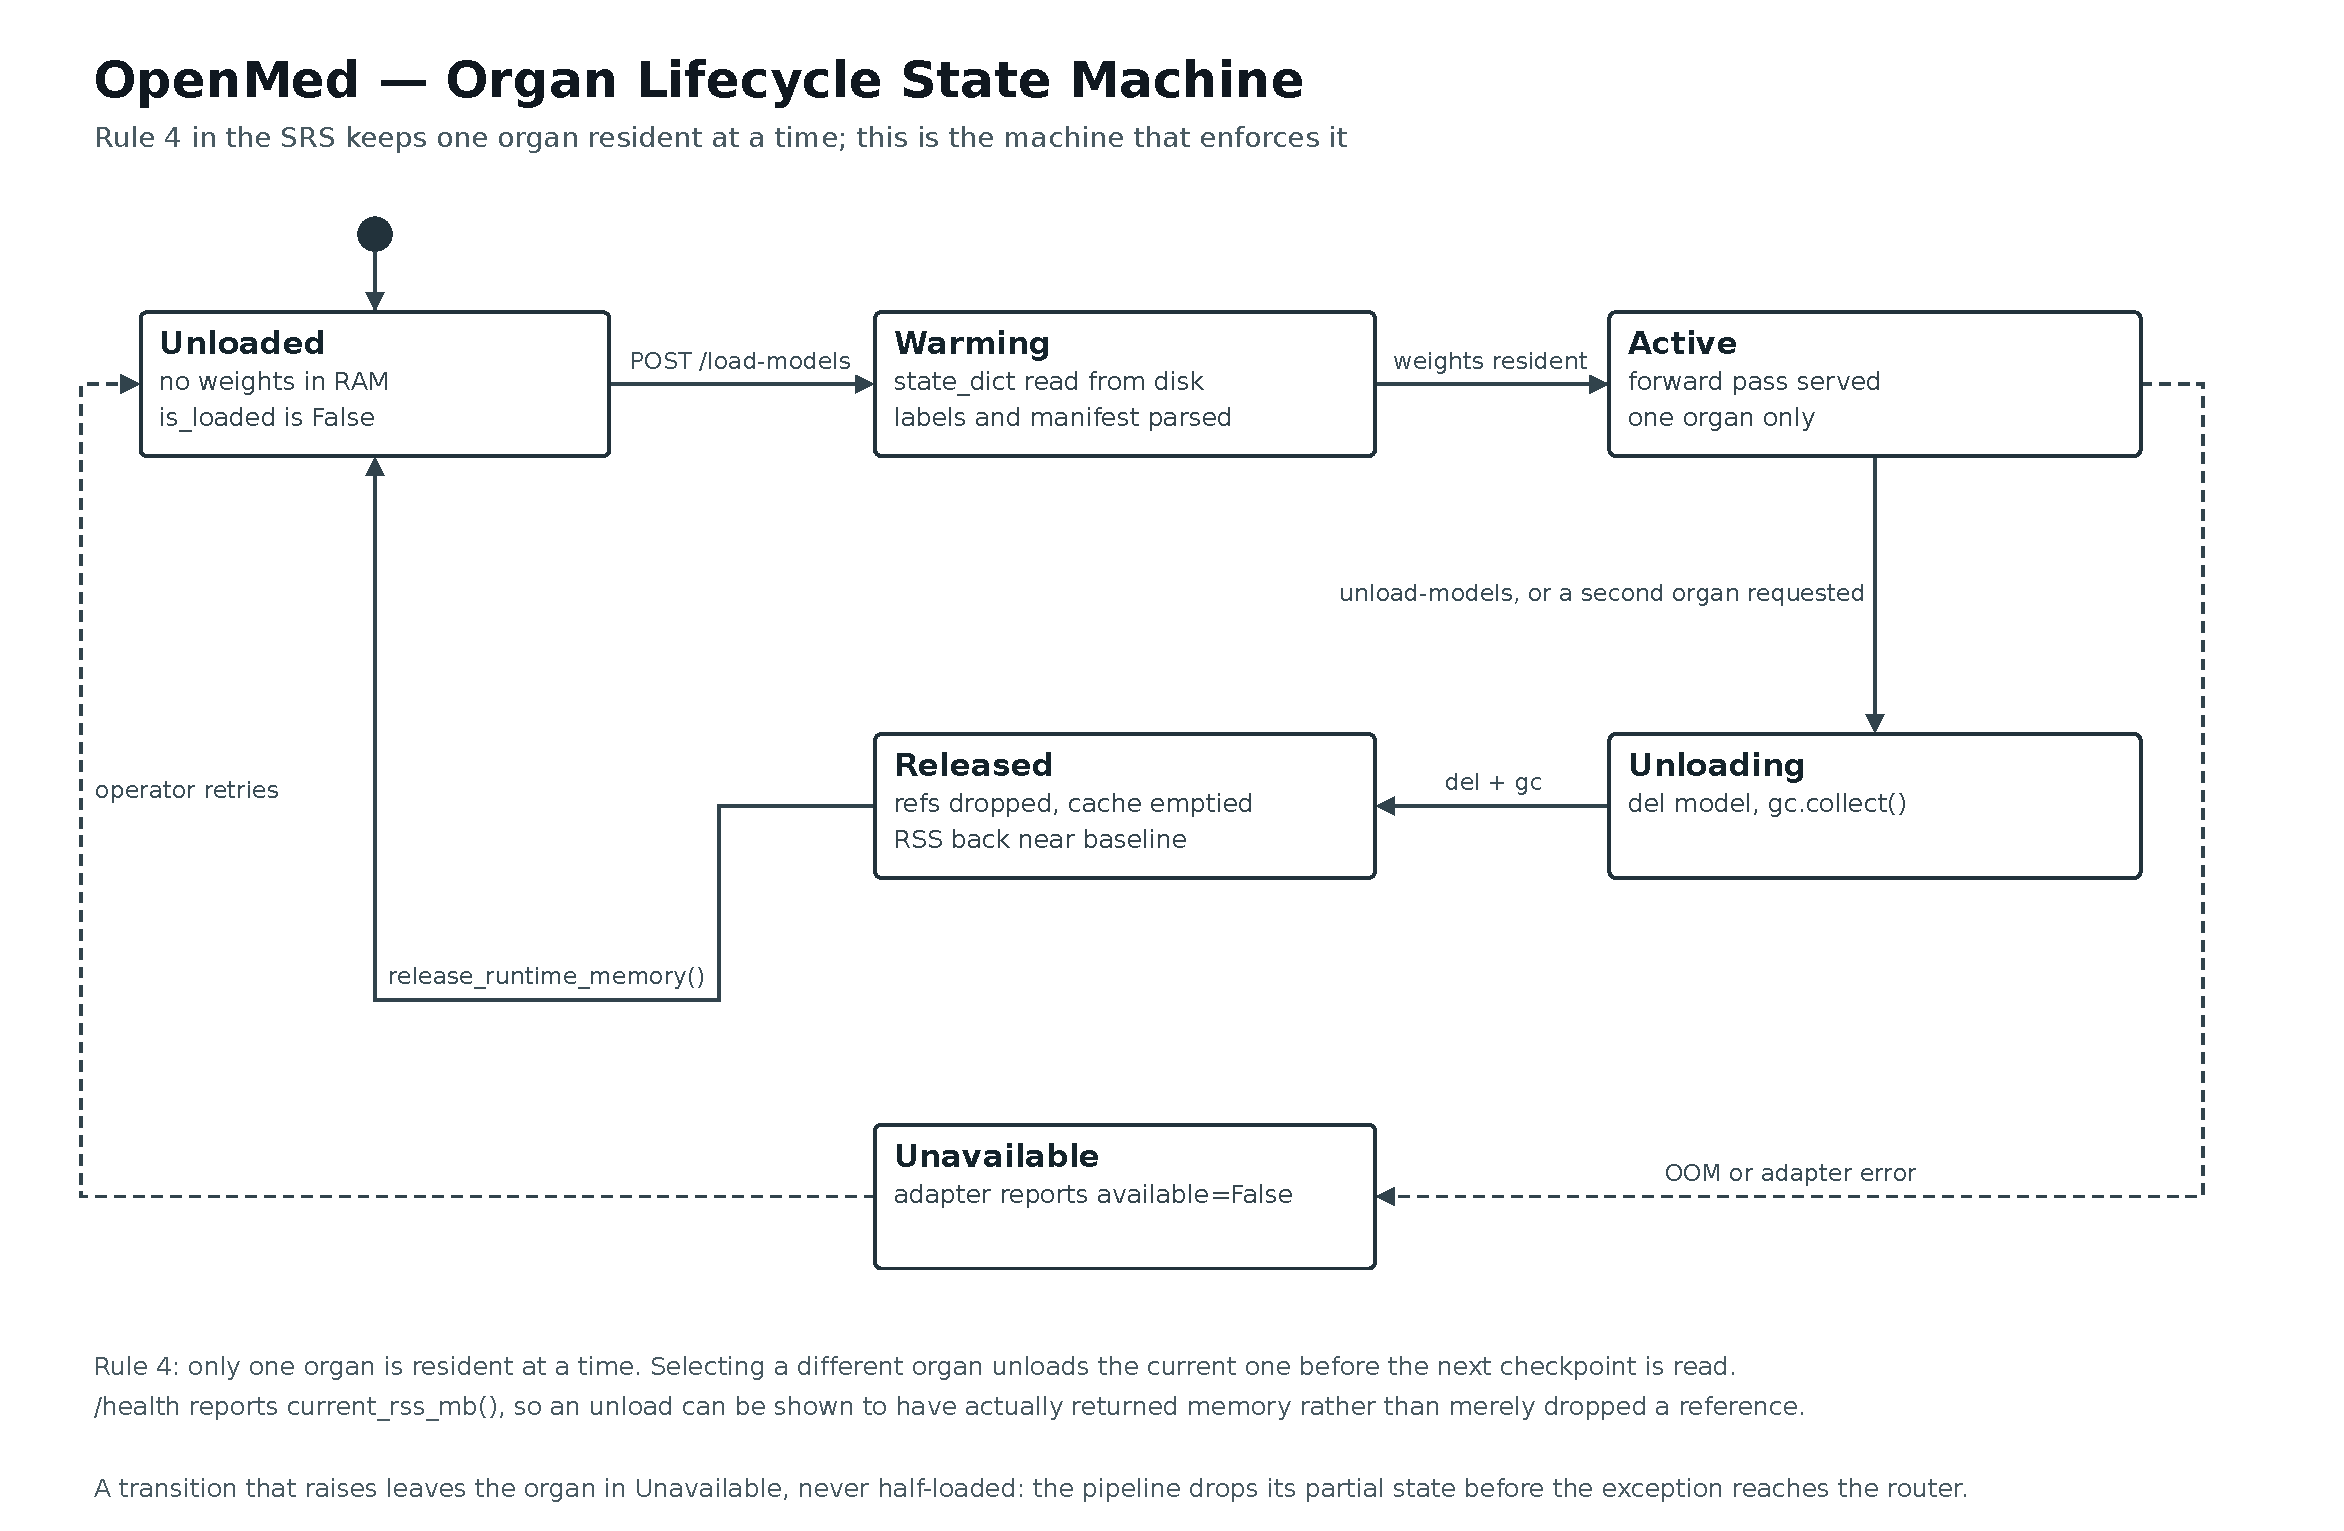
\includegraphics[width=\textwidth]{16_state_machine.pdf}
    \caption{Organ Lifecycle State Machine from Unloaded to Released and Garbage Collection}
    \label{fig:state_machine}
\end{figure}

\subsubsection{Class Diagram}
The inference-side classes only. Training modules (datasets, split planners, augmentation policy) are deliberately absent because they never ship inside the service. Composition marks the lung pipeline that owns both of its model wrappers; generalization marks the analyze response that extends the classification response.

\begin{figure}[H]
    \centering
    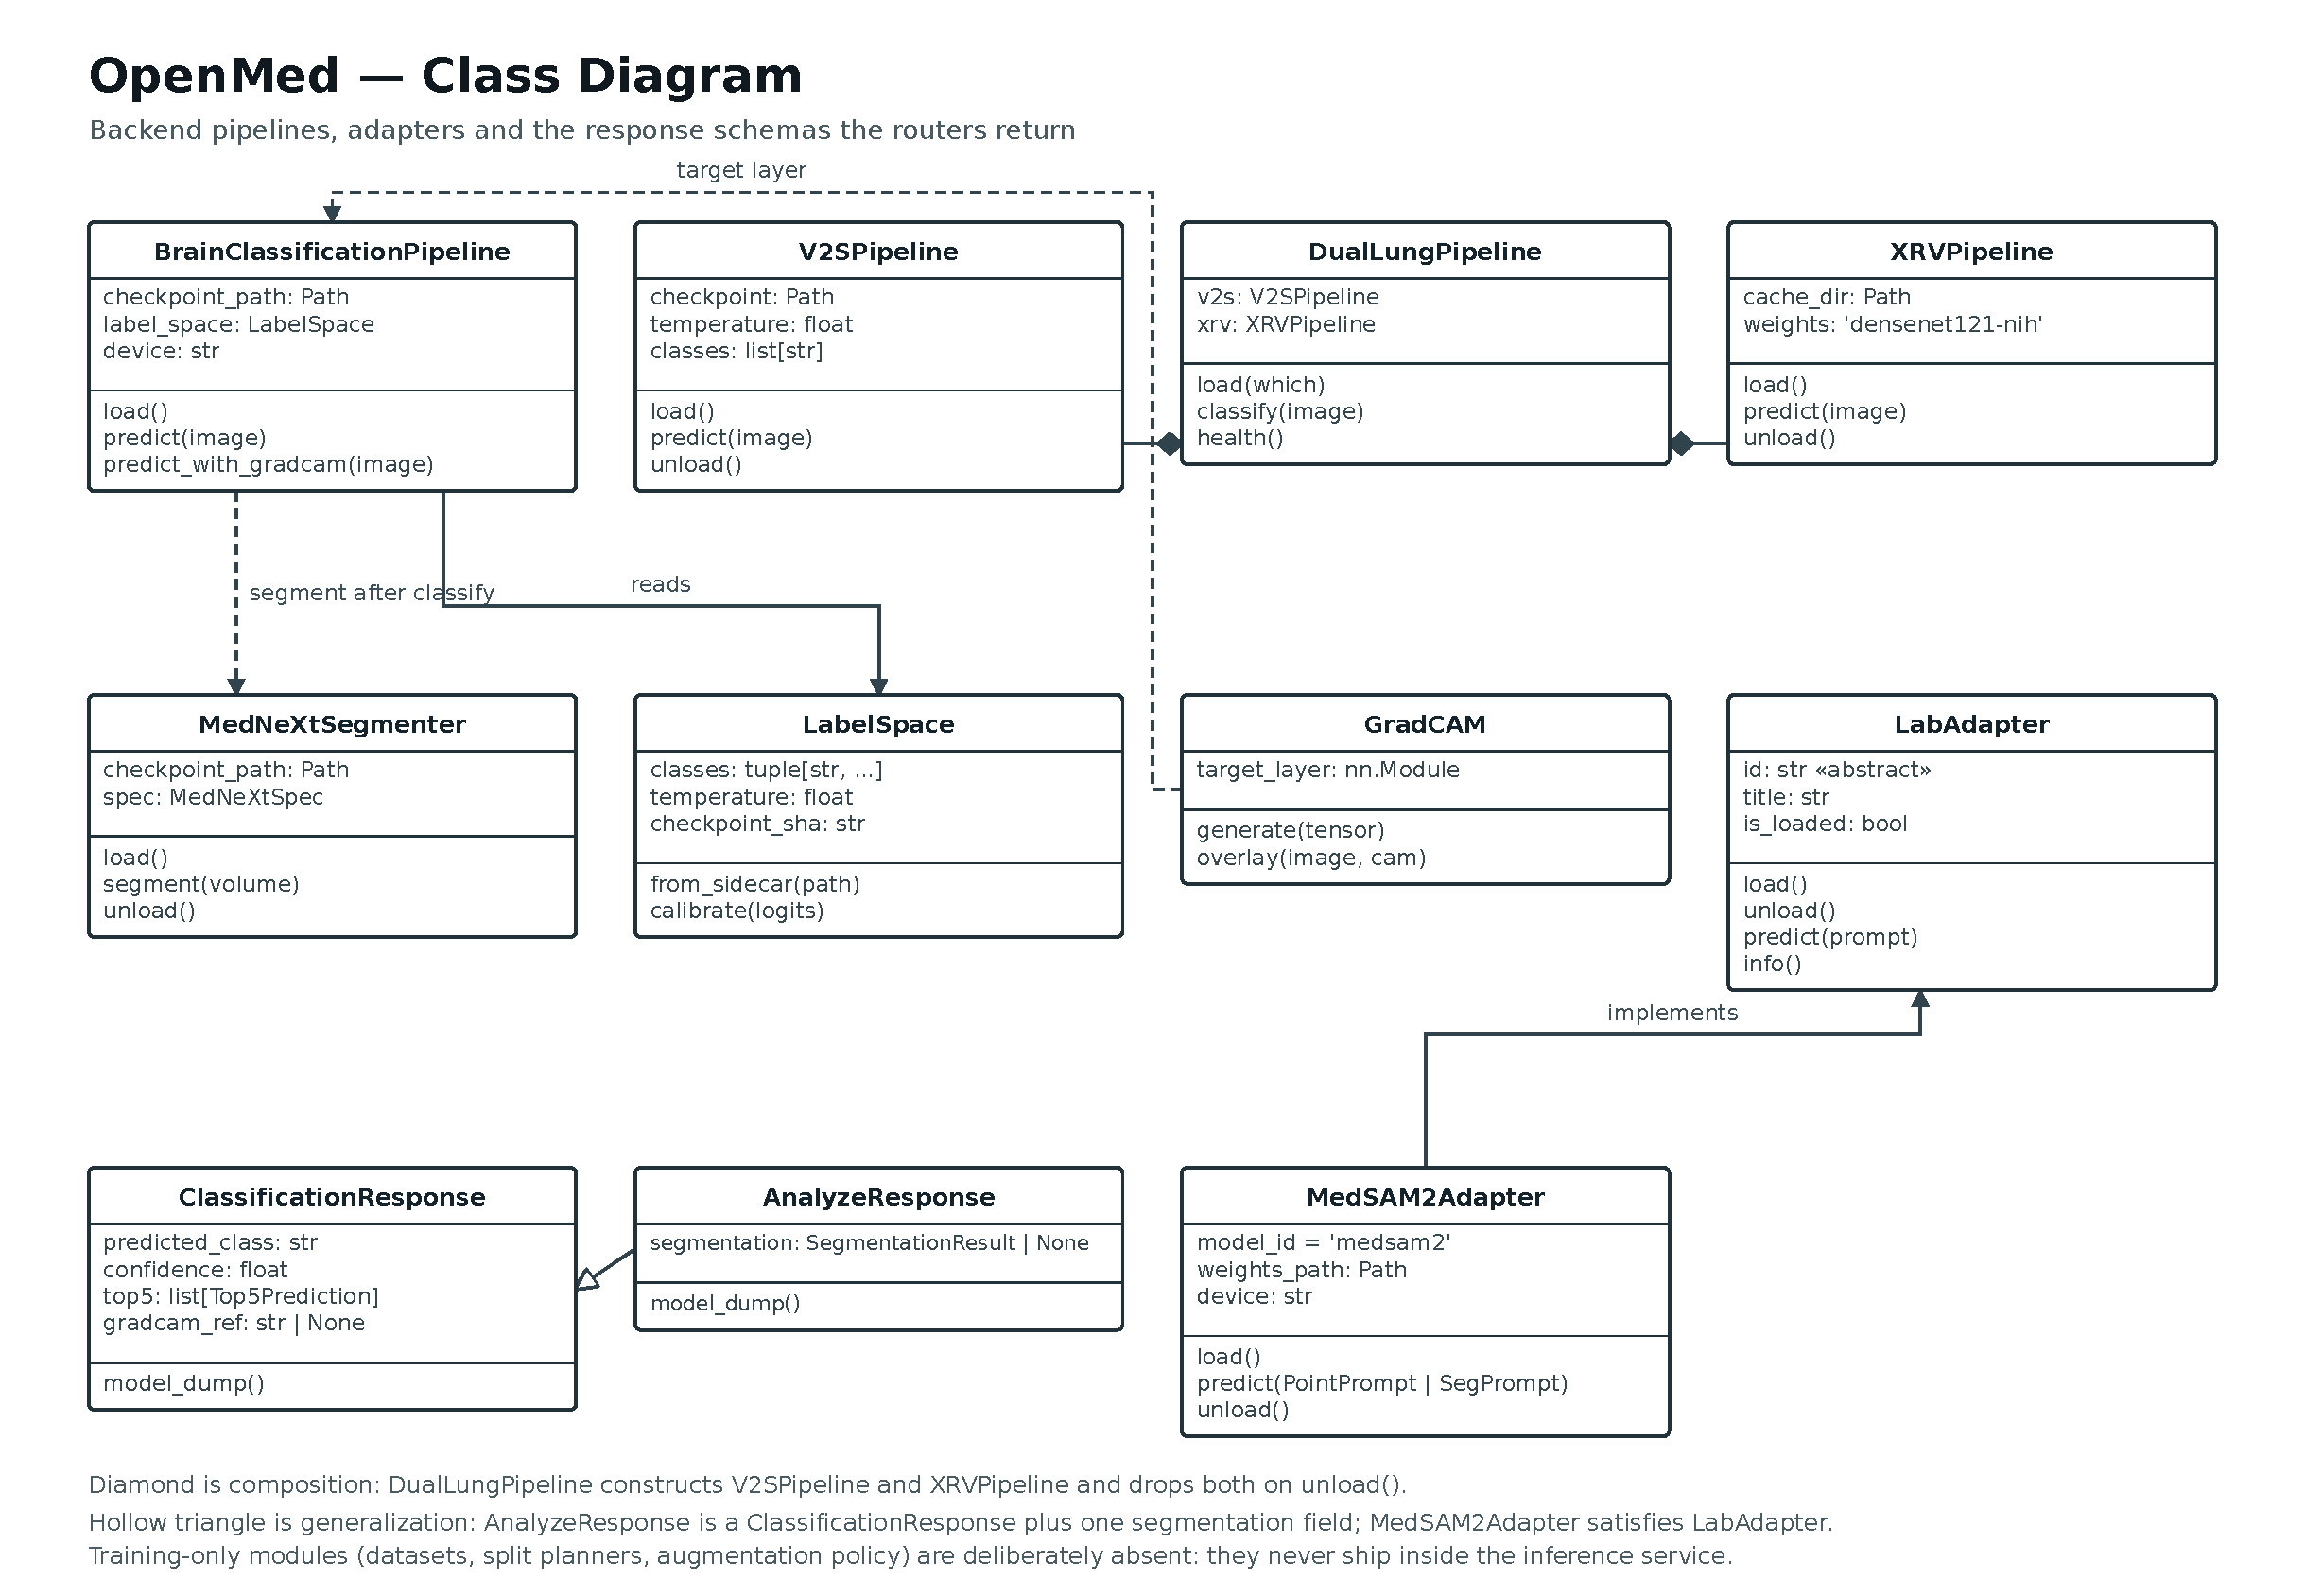
\includegraphics[width=\textwidth]{17_class_diagram.pdf}
    \caption{Class Diagram of Backend Pipelines, Model Adapters and Pydantic Response Schemas}
    \label{fig:class_diagram}
\end{figure}

\subsubsection{Data Flow Diagram}
Level 0 shows the platform as a single process because the clinician sees a single workstation. Level 1 breaks that process into ingest, classify, segment and report over the four stores the audit trail needs. The audit log is appended by every process; its four inbound flows are stated in the figure footer rather than drawn.

\begin{figure}[H]
    \centering
    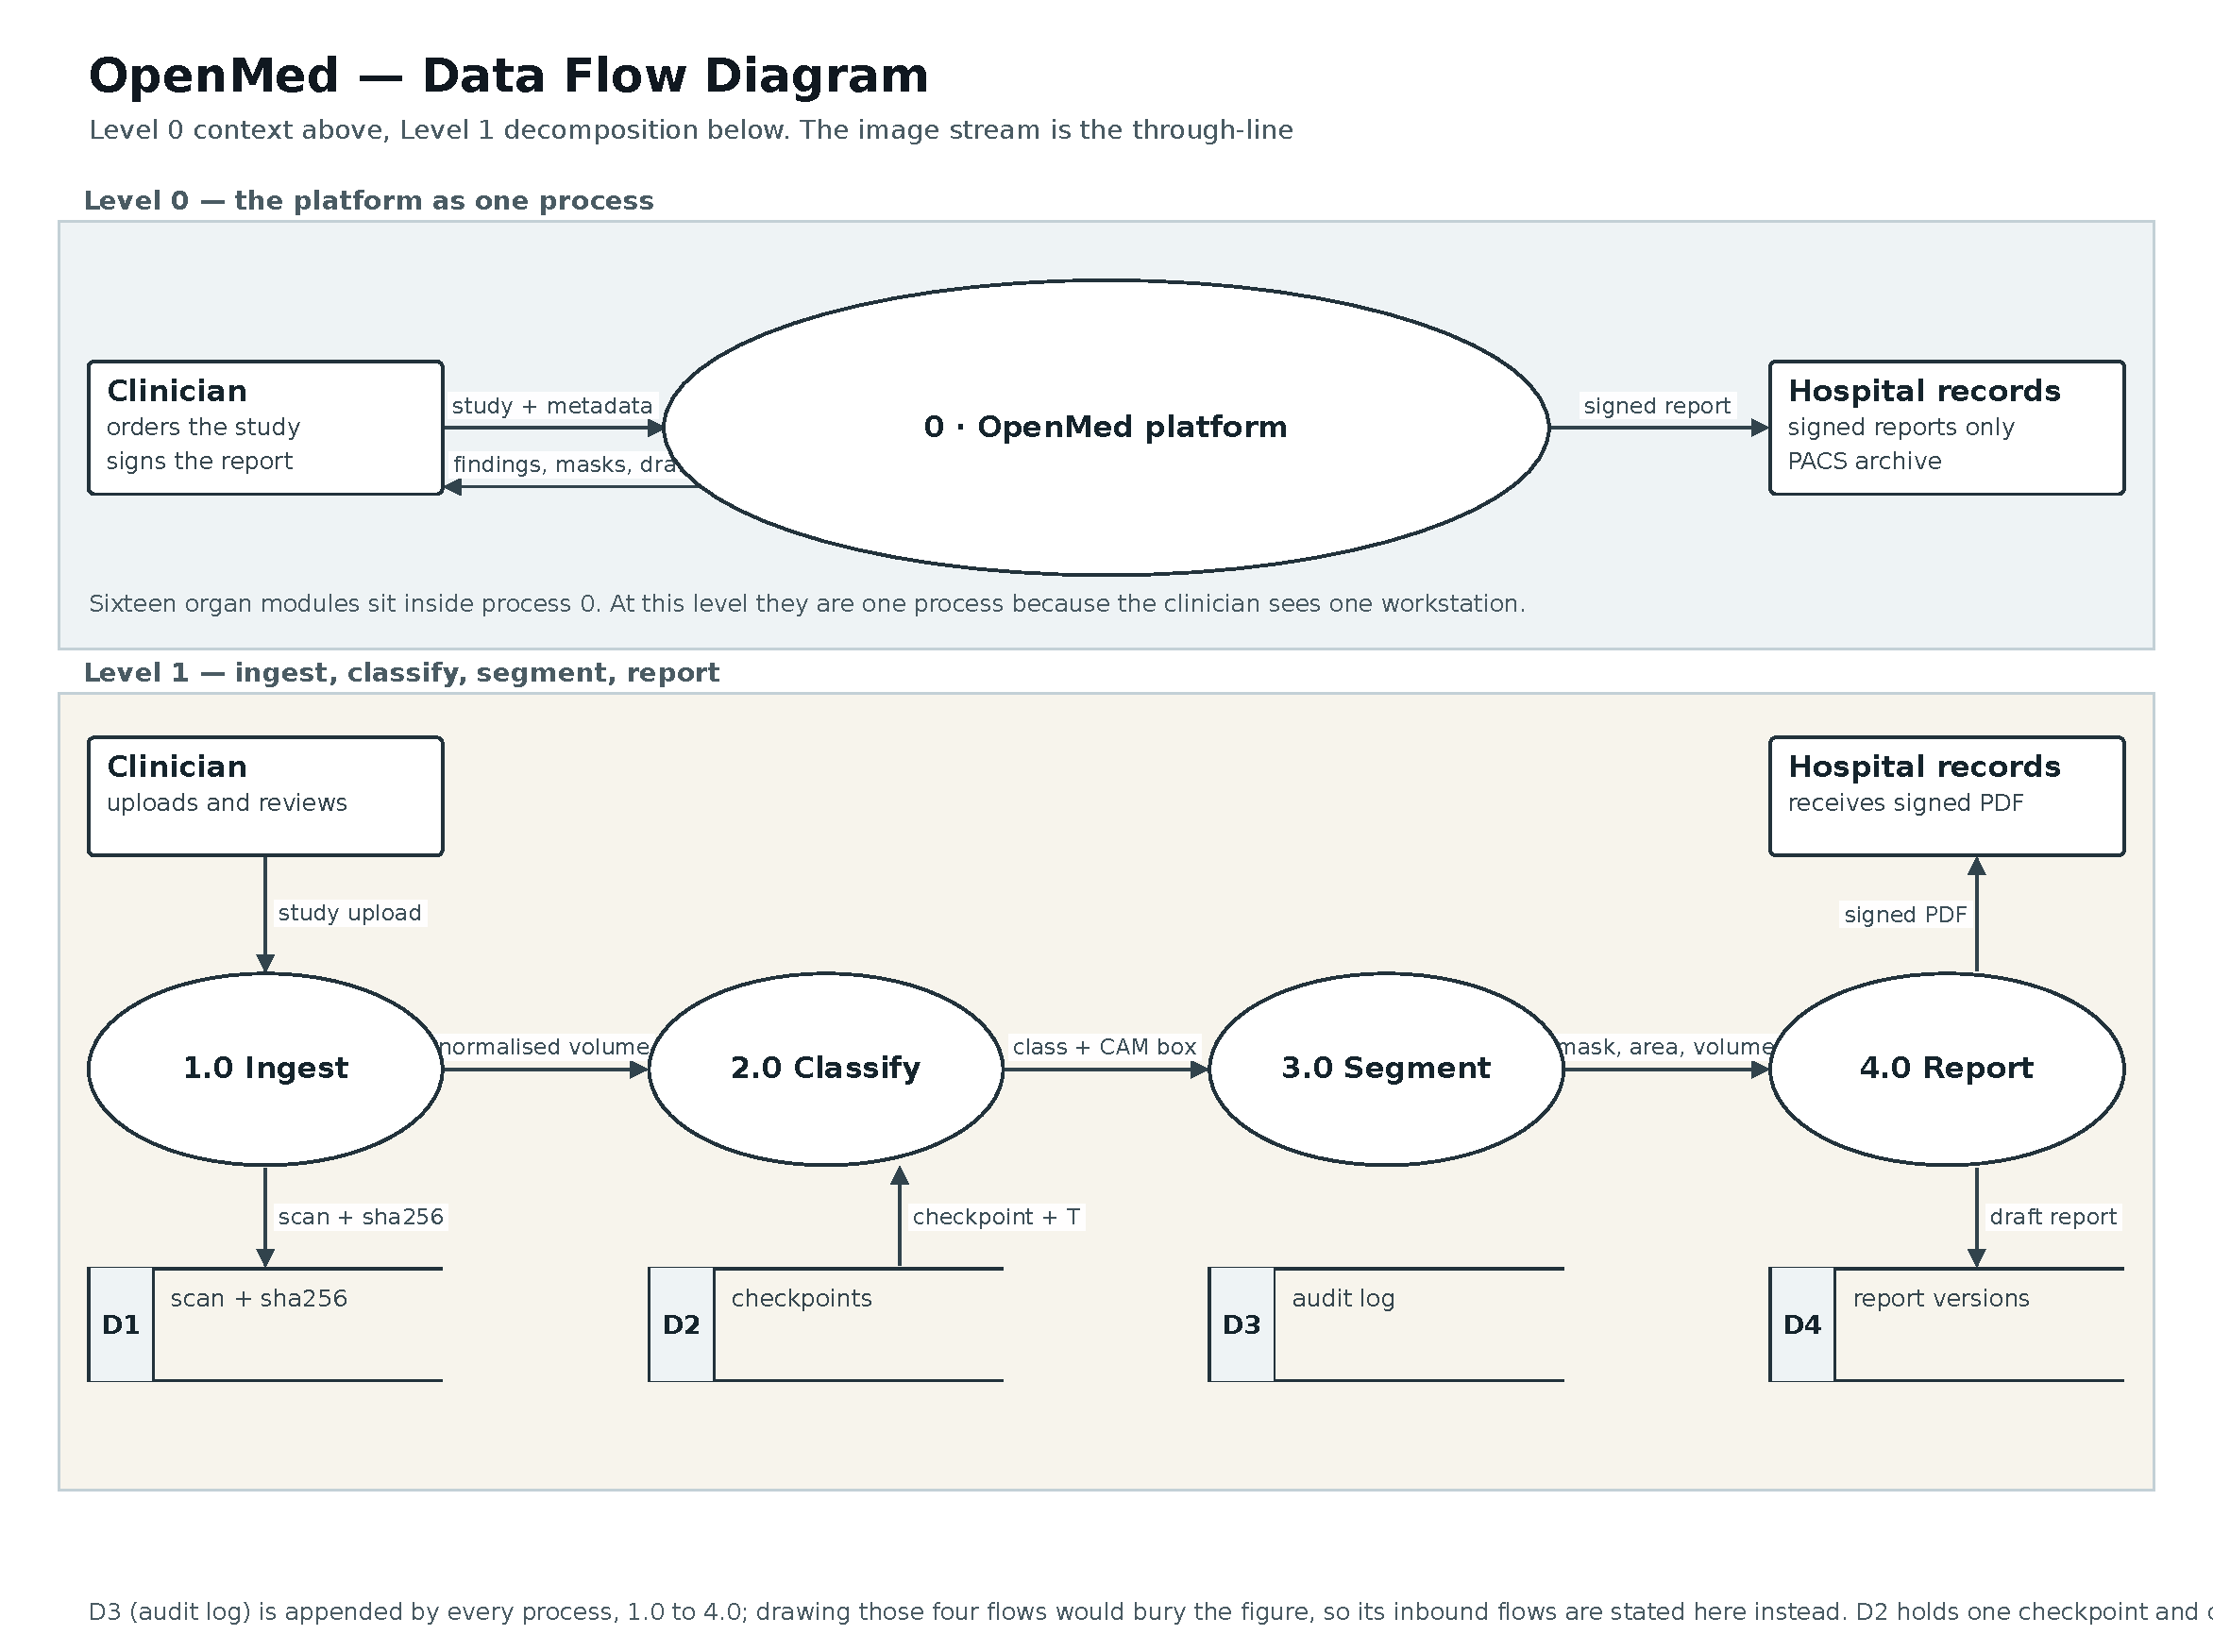
\includegraphics[width=\textwidth]{18_data_flow_diagram.pdf}
    \caption{Data Flow Diagram, Level 0 Context and Level 1 Decomposition}
    \label{fig:data_flow_diagram}
\end{figure}

\subsubsection{Database Diagram}
The physical schema behind the ER model, with SQL types, key constraints, and the indexes the query paths need. Release 1.0 targets SQLite for a single clinic; the same DDL runs on PostgreSQL unchanged apart from the serial column type. The report and audit tables are append-only by policy, and the application role holds no update or delete grant on the audit log.

\begin{figure}[H]
    \centering
    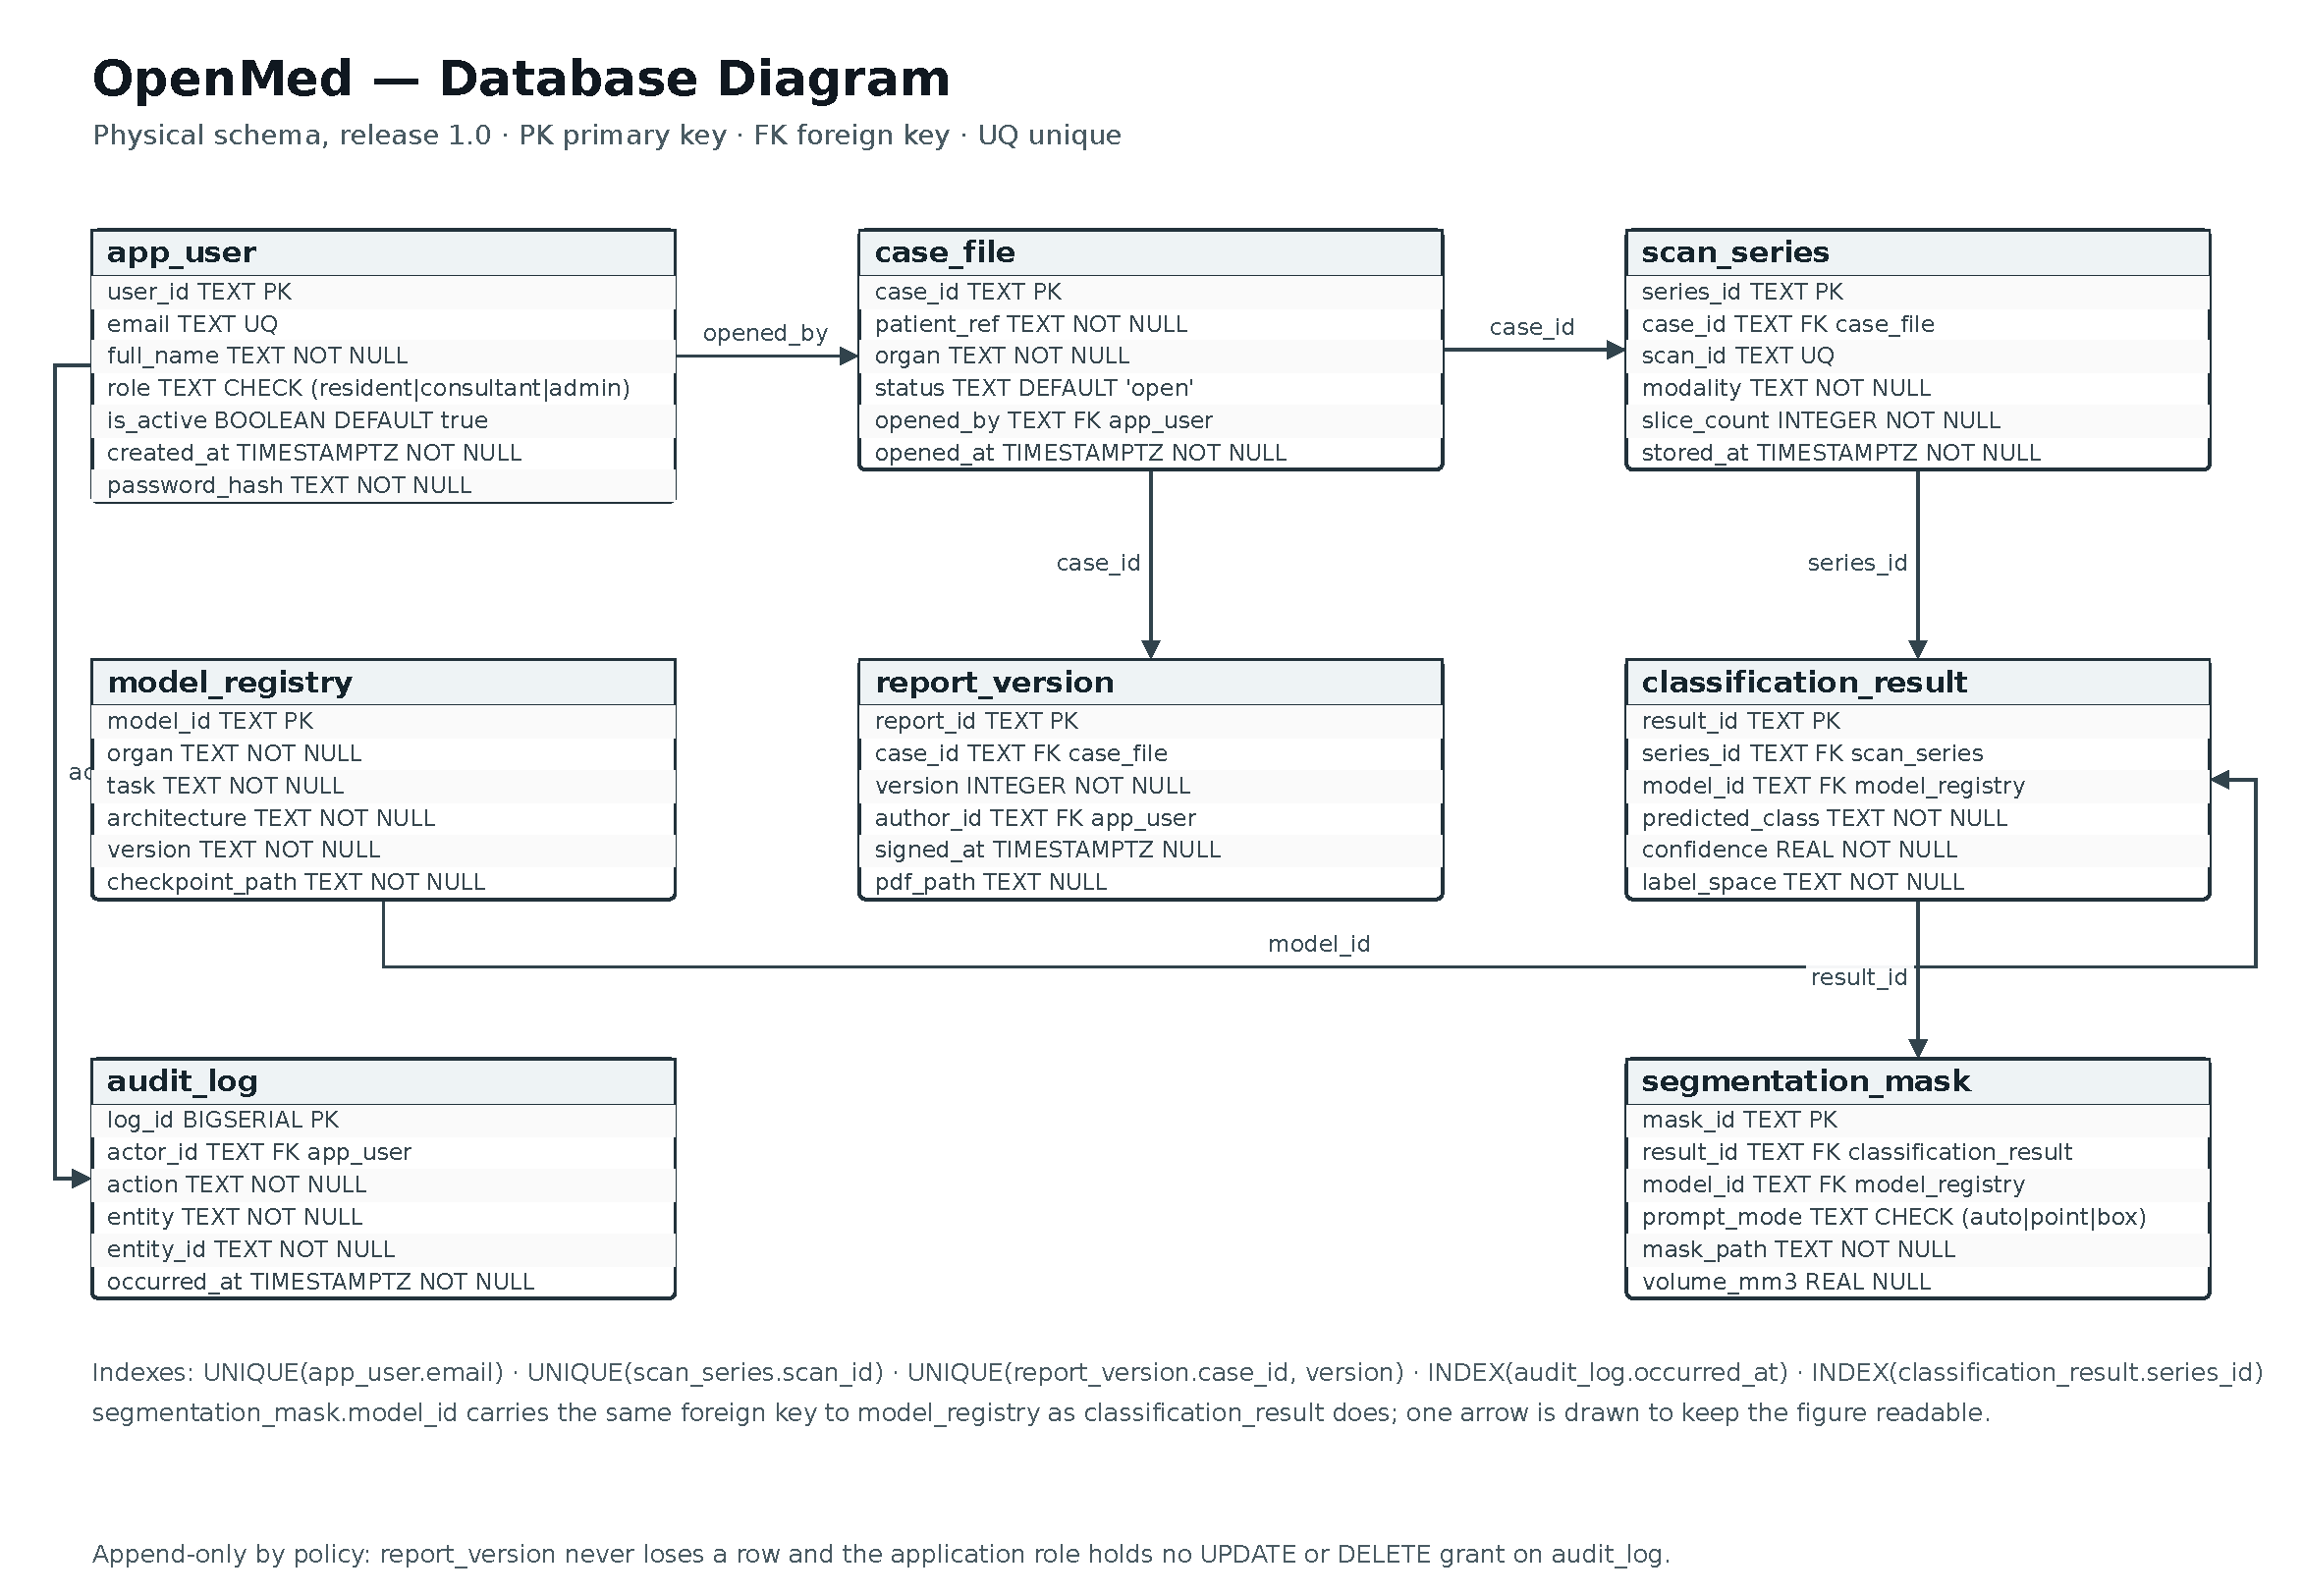
\includegraphics[width=\textwidth]{19_database_diagram.pdf}
    \caption{Database Diagram with Key Constraints and Query Indexes}
    \label{fig:database_diagram}
\end{figure}

% ----------------------------------------------------------------------
% REFERENCES
% ----------------------------------------------------------------------
\addcontentsline{toc}{section}{References}
\section*{References}
\begin{enumerate}[leftmargin=1.5em]
    \item Clinical Radiology UK Workforce Census Report. The Royal College of Radiologists (RCR), 2024. Available: \url{https://www.rcr.ac.uk/our-services/audit-and-quality/workforce-census/clinical-radiology-workforce-census/}
    \item European Society of Radiology (ESR). Radiologists workforce distribution and diagnostic density in European healthcare systems, 2024. Available: \url{https://www.myesr.org/}
    \item M. Chavoshi, S. Zamani, and S. A. Mirshahvalad, "Diagnostic performance of deep learning models versus radiologists in COVID-19 pneumonia: A systematic review and meta-analysis," \textit{Clinical Imaging}, vol. 107, p. 110092, 2024.
    \item M. E. H. Chowdhury et al., "Can AI Help in Screening Viral and COVID-19 Pneumonia?" \textit{IEEE Access}, vol. 8, pp. 132665--132676, 2020.
    \item O. Ronneberger, P. Fischer, and T. Brox, "U-Net: Convolutional Networks for Biomedical Image Segmentation," in \textit{MICCAI 2015}, LNCS 9351, pp. 234--241, 2015.
    \item N. Ravi et al., "SAM 2: Segment Anything in Images and Videos," \textit{arXiv preprint arXiv:2408.00714}, 2024.
    \item J. Wasserthal et al., "TotalSegmentator: Robust Segmentation of 104 Anatomic Structures in CT Images," \textit{Radiology: Artificial Intelligence}, vol. 5, no. 5, p. e230024, 2023.
    \item M. Tan and Q. V. Le, "EfficientNetV2: Smaller Models and Faster Training," in \textit{ICML 2021}, PMLR 139, pp. 10096--10106, 2021.
    \item J. Cohen et al., "TorchXRayVision: A library of chest X-ray datasets and models," in \textit{MIDL 2022}, PMLR 172, 2022.
    \item OpenMed GitHub Repository and Technical Specification. Available: \url{https://github.com/H0NEYP0T-466/OpenMed}
\end{enumerate}

\end{document}